\section{Introduction}
\label{sec:introduction}


In this work we introduce two new methods for the discretization of
the steady incompressible Stokes equations in three space dimensions.
Let $\Omega \subset \rr^3$ be an open bounded domain with
Lipschitz boundary $\partial \Omega$ that is split into the Dirichlet
boundary $\GammaD$ and outflow boundary
$\GammaN$. The Stokes system for
the fluid {\em velocity} $u$ and the {\em pressure} $p$
is given by
\begin{subequations}\label{eq::stokes}
\begin{alignat}{2} 
  -\div(\nu \eps(u)) + \nabla p & = f && \quad \textrm{in } \Omega, \label{eq::stokes-a} \\
  \div u &=0 && \quad \textrm{in } \Omega, \label{eq::stokes-b}\\
  u &= 0 &&\quad \textrm{on } \GammaD, \label{eq::stokes-c}\\
  (-\nu\eps(u) + p I)n &= 0 &&\quad\textrm{on } \GammaN,\label{eq::stokes-d}
\end{alignat}
\end{subequations}
where $\eps(u) := (\nabla u + \nabla u ^\trans)/2$ is the symmetric
gradient, $f: \Omega \rightarrow \rr^3$ is an external body force,
$\nu$  is twice the kinematic viscosity,
$n$ is the outward unit normal vector and
$I\in\rr^{3\times 3}$ is the identity matrix.
We assume that both $\GammaD$ and $\GammaN$ have positive boundary
measure, and any rigid displacement vanishing on $\Gamma_D$
vanishes everywhere in~$\Omega$. (As usual, when $\Gamma_N$ is empty the pressure
space must be adapted to obtain a unique 
pressure~\cite{girault2012finite}, but we omit this case for simplicity.)
Next, define the {\em viscous stress tensor} \cite{LandaLifsh59}
by $\sigma = \nu \eps(u)$ and the {\em vorticity} by  $\omega =
\curl u$. Using them,  we can rewrite the above system as
\begin{subequations}
  \label{eq::mixedstressstokes}
  \begin{alignat}{2}
  \label{eq::mixedstressstokes-a}
  \nu^{-1}{\dev{\sigma}} - \nabla u + \kappa(\omega) & = 0  &&\quad  \textrm{in } \Omega,  \\
  \label{eq::mixedstressstokes-b}
  -\div  \sigma + \nabla p & = f  &&\quad  \textrm{in } \Omega,  \\
 \label{eq::mixedstressstokes-c} 
 \sigma - \sigma^\trans & = 0 && \quad \textrm{in } \Omega,  \\
  \label{eq::mixedstressstokes-d} 
  \div u &=0 &&\quad  \textrm{in } \Omega, \\
  \label{eq::mixedstressstokes-e}
  u &= 0 &&\quad \textrm{on } \GammaD, \\
  (\sigma - p I)n &= 0 &&\quad\textrm{on } \GammaN.
  \label{eq::mixedstressstokes-f}
 \end{alignat}
\end{subequations} 
Here we used the deviatoric part of the tensor $\tau$ given by
$
  \dev{\tau} := \tau - \frac{1}{3}\trace{\tau} I,
$
the matrix trace $\trace{\tau} := \sum_{i=1}^3 \tau_{ii}$, and the
operator $  \kappa: \rr^{3} \to \{\tau \in \rr^{3 \times 3}: \tau +
\tau^{\trans} = 0 \}$ defined by 
\begin{align*}
  \kappa(v) =
  \frac 1 2 
  \begin{pmatrix}
    0 & -v_3 & v_2 \\
    v_3 & 0 & -v_1 \\
    -v_2 & v_1 & 0
  \end{pmatrix}.
\end{align*}
Note the obvious identities
\begin{equation}
  \label{eq:kappa-identities}
  \nabla v = \eps(v) + \kappa(\curl v),
  \qquad
  2 \kappa(v) w = v \times w,
\end{equation}
for vector fields $v$ and $w$ (the first of which was already  used in~\eqref{eq::mixedstressstokes-a}).
We will refer to system~\eqref{eq::stokes} as the primal
formulation and system~\eqref{eq::mixedstressstokes} as the mixed formulation.


The literature on discretizations of \eqref{eq::stokes} and
\eqref{eq::mixedstressstokes} is too vast to list here.  The
relatively  recent quest for exactly divergence-free velocity
solutions and pressure-independent a~priori error estimates for
velocity, often referred to as pressure robust
estimates~\cite{linke2014role, 2016arXiv160903701L}, has rejuvenated
the field.  A recurring theme in this vast literature, from the early
non-conforming method of~\cite{CrouzRavia73} to the more
recent~\cite{LS_CMAME_2016}, is the desire to improve computational
efficiency by minimizing inter-element coupling. However, less studied
are its side effects on stability when
 the actual physical flux replaces 
the often-used simplified diffusive flux, i.e., when
\begin{align} \label{eq::nablavseps}
  -\div(\nu \eps(u))
  \quad \textrm{replaces} \quad
  -\div(\nu \nabla u),
\end{align}
even though an early work~\cite{Falk91} cautions how the lowest order
method of~\cite{CrouzRavia73} can become unstable when doing so.
Such instabilities arise because the larger null space of $\eps$
necessitates increased inter-element coupling (as explained in more
detail below) and are manifested in certain lowest order cases with
insufficient inter-element coupling.  In this work, focusing on the
lowest order case, we identify new stable finite element methods, with
the minimal necessary inter-element coupling, that yield exactly
divergence-free and pressure robust velocities.
New methods based on both the primal and the mixed
formulations are designed.


Yet another reason for focusing on the lowest order case is its
utility in preconditioning. Roughly speaking, a common strategy for
preconditioning high order Stokes discretizations involves combining
local (high order) error dampers via, say block Jacobi or other
smoothers, with a global (low order) error corrector such as multigrid
(or even a direct solver) applied  to the smaller lowest order
discretization.  From this point of view, it is desirable to have
stable low order versions (that remain stable
under~\eqref{eq::nablavseps}) of high order methods for design of
preconditioners, an interesting topic which we shall not touch upon
further in this paper.



To delve deeper into the mechanics of the above-mentioned instability,
consider the kernel of $\eps$, consisting of rigid displacements of the form
$x\to a + b \times x$ with $a,b\in\rr^3$. Reasonable methods
approximating the operator $-\div(\nu \eps(u))$ produce element
matrices whose nullspaces contain these rigid displacements. Ideally, when
these element-wise rigid displacements are subjected to the inter-element
continuity conditions of the discrete velocity space, they should
equal element-wise restrictions of a global rigid displacement on $\Omega$
(which can then be eliminated by boundary conditions).  However, if
the inter-element coupling in the discrete velocity space is so weak
to allow for the existence of a $u$ in it that does not equal a global
rigid displacement on $\Omega$ even though $u|_T$ is a rigid displacement on every
mesh element~$T$, then instabilities can arise~\cite{Falk91}.

The discrete velocity space we have in mind is the lowest order
(piecewise linear) $H(\div)$-conforming Brezzi-Douglas-Marini ($\BDM$)
space~\cite{brezzi2012mixed}.  (A basic premise of this paper is the
unquestionable utility of $H(\div)$-conforming velocity spaces to
obtain exactly divergence-free discrete Stokes velocity fields, well
established in prior works~\cite{cockburn2005locally,
  cockburn2007note, LS_CMAME_2016,mcsI, mcsII}). Hence, to understand
how to avoid the above-mentioned instability while setting velocity in  the $\BDM$
space, we ask the following question: {\em how many coupling degrees of
  freedom} (\dofs) {\em are needed to guarantee that two rigid displacements
$u_\pm$, given respectively on two adjacent elements $T_\pm$,
coincide on the common interface $F = \partial T_+ \cap \partial T_-$?}

\begin{figure}
  \centering
  \includegraphics[width=0.9\textwidth, clip = true, trim = 1cm 0 0 0 ]{rigid2.pdf}
  \caption{Configurations of adjacent elements after
    deformation by piecewise rigid displacements of two adjacent elements $T_\pm$.}
  \label{fig::motions}
\end{figure}


The pictorial representations of the deformations created by $u_\pm$
in Figure~\ref{fig::motions} lead to the answer. Three of the pictured
deformations are just translations (generated by the $a$-vector in $a
+ b \times x$).  For a unit vector $b$, letting $R^b_\theta$ denote
the unitary operator that performs a counterclockwise rotation by
angle $\theta$ around $b$, it is easy to see that $R^b_\theta x = x +
\theta (b \times x) + \mathcal{O}(\theta^2)$ as $\theta \to 0$.
Therefore the deformation created by the rigid displacement $b \times
x$ can be viewed as an infinitesimal rotation about~$b$. These
deformations are portrayed in Figure~\ref{fig::motions} as rotations
about three linearly  independent~$b$-vectors.  The first row in
Figure~\ref{fig::motions} illustrates deformations generated by
piecewise rigid displacements which are given by two $b$-vectors
coplanar with $F$ and an $a$-vector normal to $F$.  These rigid
displacements are forbidden in the $\BDM$ space. Indeed, 
recall~\cite{brezzi2012mixed} that the $\BDM$ \dofs\ on the facet
  $F$ are given by the linear functionals
  $ u \mapsto \int_F u \cdot n ~q \ds$ for all linear polynomials $q$  on $F$,
  where $n$ is a normal vector on $F$. These represent three \dofs\ illustrated in
  left diagram of Figure~\ref{fig::dofs}.
  If these three \dofs\ coincide for two
rigid displacements $u_{\pm}$, then the corresponding normal component must
be continuous on $F$. This continuity forbids the
above-mentioned deformations to be generated by 
elements of the $\BDM$ space. We summarize this by saying that the  rigid displacements
portrayed in the first row of Figure~\ref{fig::motions}
are ``controlled'' by the three $\BDM$ \dofs~of the facet $F$ which
are illustrated in the left diagram of Figure~\ref{fig::dofs}.



It remains to control the rigid displacements of the second row of
Figure~\ref{fig::motions} using three additional \dofs\ per facet.
To this end, our new methods have two additional spaces: (i) one that
approximates the in-plane components of the velocity on facets,
illustrated in the middle diagram of Figure~\ref{fig::dofs}, used to
control the first two rigid displacements in the second row of
Figure~\ref{fig::motions}; and (ii) a second space, schematically
indicated in the last diagram of Figure~\ref{fig::dofs}, that controls
the third deformation in the second row of Figure~\ref{fig::motions}.
The latter deformation arises from piecewise rigid displacements of the form
$u_\pm = b_\pm \times x$ with $b_\pm$ collinear to $n$, a unit normal
of $F$.  Since $\curl(b_\pm \times x) = 2 b_\pm$, we can make the two
rigid displacements coincide on $F$ by requiring continuity of
$n \cdot \curl u_\pm$. While continuity of $n \cdot \curl u$
certainly holds if $u$ is the exact Stokes velocity, it does not
generally hold for $u$ in $\BDM$. Hence, keeping in view that
$\omega = \curl u$ represents vorticity, {\em we incorporate this
  constraint in our new methods by approximating vorticity $\omega$ in the lowest
  order Raviart-Thomas space.} This is our second additional space.
Its single {\tt dof}  per facet  is shown schematically in the last diagram of
Figure~\ref{fig::dofs}.

\begin{figure}
  \centering
  \includegraphics[width=0.9\textwidth, clip = true, trim = 1cm 0 0 0 ]{dofs.pdf}
  \caption{Classification of facet \dofs\ in our new methods into three types:
    (1) normal velocity components in the form of  $\BDM$ facet dofs,
    (2) tangential facet velocities,
    (3) normal vorticity as $\RT$ facet dof. 
  }
  \label{fig::dofs}
\end{figure}

In the first part of the paper we will employ these additional spaces
to construct a novel HDG method to approximate~\eqref{eq::stokes} and
present a detailed stability and error analysis.
HDG methods have become popular ever since its introduction in~\cite{cockburn2009unified} which showed  how interface variables,
or facet variables, 
can be effectively used to construct DG schemes amenable to
static condensation.
In the method presented here, the interface variable approximates the
tangential components of the velocity.
The key technical
ingredient in the analysis that reflects the insight garnered from the
above pictorial discussion is a discrete Korn-like inequality for the
$\BDM$ space
% piecewise $H^1$ fields with continuous normal components
(see Lemma~\ref{lemma::korn} below, 
and the version with interface variables  in
Lemma~\ref{lem::korn_hdg}).

The second part of this work discusses the derivation of a novel mixed
method for the approximation of \eqref{eq::mixedstressstokes} and is
motivated by our previous two papers~\cite{mcsI,mcsII} and the many
other works on discretizing~\eqref{eq::mixedstressstokes} such as
\cite{Farhloulcanadian, MR1231323, MR1464150, MR1934446}. In
\cite{mcsII} we derived the ``\underline{M}ass-\underline{C}onserving \underline{S}tress-yielding'' (MCS)
formulation where the symmetry of $\sigma$ was incorporated in a weak sense
by means of a Lagrange multiplier that approximates
$\omega = \curl u$. While the $\omega$ there was approximated using
element-wise linear (or higher degree) functions {\em without} any
inter-element continuity requirements, the new mixed method we propose
here will approximate $\omega$ in the lowest order Raviart-Thomas
space instead.  The lowest order case that was proved to be stable
in~\cite{mcsII} had nine coupling \dofs\ per facet. We are able
to reduce this number to the minimal six (the dimension of rigid
displacements) in this paper.
This minimal coupling was achieved earlier in~\cite{TaiWinth06} using
a bubble-augmented velocity space which is a subspace of a degree-four
vector polynomial space. Since higher degrees necessitate more
expensive integration rules, we offer our simpler elements as an
alternative.


Other methods that approximate the operator $\div(\nu \nabla u)$,
such as~\cite{CrouzRavia73,LS_CMAME_2016, mcsI}, are able to reduce
the number of coupling \dofs\ per facet even further. Since our focus
here is on methods that approximate $\div(\nu \eps( u))$, we restrict
ourselves to a brief remark on this.  Since the kernel of $\nabla$ (applied to vector fields) is
three dimensional, we expect the minimal number of coupling \dofs\ per
facet to be three when approximating $\div(\nu \nabla u)$. A method
with this minimal coupling was
achieved early by~\cite{CrouzRavia73}.  To also obtain pressure robust and
exactly divergence-free solutions, prior works~\cite{LS_CMAME_2016,
  mcsI} settled for a slightly higher five coupling \dofs\ per facet
in the lowest order case.  It is now known that this can be improved
by employing the technique of ``relaxed
$H(\div, \Omega)$-conformity,''
see~\cite{ledlehrschoe2017relaxedpartI,ledlehrschoe2018relaxedpartII},
which results in a method with the minimal three coupling \dofs\ per facet and yet,
thanks to a simple post-processing, provides optimal convergence
orders and pressure robustness.
While on the subject of coupling \dofs, an 
  explanation of our focus on three-dimensional (3D) domains is in order.
  On two-dimensional (2D)
domains, the space of rigid displacements only has three
dimensions. In the lowest order 2D case, $\BDM$ space provides two coupling
\dofs\ per facet edge, and the space of tangential facet velocities
adds one more coupling degree of freedom. Thus the minimal facet
coupling (of three \dofs) needed to eliminate the rigid
displacements are more immediate in 2D case when compared to the 3D
case, which is why restrict to the 3D case henceforth.



The new HDG method and the new mixed method proposed in this paper
both have the same coupling \dofs, the same velocity convergence orders
and the same structure preservation properties like pressure robustness
and mass conservation. On closer comparison, two advantages of the
mixed method are notable. One is its direct approximation of viscous
stresses. Another is the absence of any stabilization parameters in
it. In fact, in our numerical studies, the conditioning of a matrix
block arising from the parameter-free mixed method was found to be better
than the analogous HDG block for all ranges of the HDG stabilization
parameter we considered.




{\bf{Outline.}} We set up general notation in
Section~\ref{sec::prelim} and continue with a description of the
variational framework used throughout the paper.  Finite element spaces, a discrete
Korn-like inequality, and resulting norm equivalences are introduced
in Section~\ref{sec::fem_ne_io}. A list of interpolation operators
into these spaces and their properties with references to literature
can also be found there. In Section~\ref{sec::hdg} we introduce and
analyze the HDG method for the primal set of equations
\eqref{eq::stokes} and in Section~\ref{sec::mcs} we do the same for
the MCS method for the mixed set of equations
\eqref{eq::mixedstressstokes}. Finally, in Section \ref{sec::numex} we
perform numerical experiments to illustrate and complement our
theoretical findings.

\section{Notation and weak forms} \label{sec::prelim}

 By $\mm$ we denote the vector space of real $3 \times 3$ matrices and
by $\kk$ we denote the vector space of $3 \times 3$ skew symmetric
matrices, i.e., $\kk = \skw(\mm)$, where $\skw \tau
= \frac{1}{2} (\tau - \tau^T)$ for $\tau \in \mm$. Further, let
$\dd = \dev{(\mm)}$. To indicate vector and matrix-valued functions on
$\Omega$, we include the range in the notation, thus while
$L^2(\Omega) = L^2(\Omega, \rr)$ denotes the space of square
integrable and weakly differentiable $\rr$-valued functions on
$\Omega$, the corresponding vector and matrix-valued function spaces
are defined by
$L^2(\Omega, \rr^3) := \left\{ u : \Omega \to \rr^3 \big| \;u_i \in
L^2(\Omega)\right\}$ and $  L^2(\Omega,\mm ) := \left\{ \tau : \Omega
\to {\mm} \big|\; \tau_{ij} \in L^2(\Omega)\right\},$ respectively.
For any ${\tilde{\Omega}} \subseteq \Omega$,  we
denote by $(\cdot,\cdot)_{\tilde{\Omega}}$ the inner product on $L^2({\tilde{\Omega}})$
(or its vector- or matrix-valued versions). Similarly, we extend this
notation and write $\| \cdot \|_{{\tilde{\Omega}}}$ for the corresponding
$L^2$-norm of a (scalar, vector, or matrix-valued) function on the domain ${\tilde{\Omega}}$. In the case ${\tilde{\Omega}} =
\Omega$ we will omit the subscript in the inner product, i.e. we have
$(\cdot,\cdot)_{\tilde{\Omega}} = (\cdot,\cdot)$ and we will use the notation
$\| \cdot \|_0 = \| \cdot \|_\Omega$.

 In addition to the differential operators we have already used, 
 $\nabla, \eps, \curl$, 
we understand $\div \Phi $ as either
$\sum_{i=1}^3 \partial_i \Phi_i$ for a vector-valued function $\Phi$,
or the row-wise divergence $\sum_{j=1}^3 \partial_j \tau_{ij}$ for a
matrix-valued function $\tau$. % The same notation is used also for the
% weak differential operator $\curl(\cdot)$. 
In addition to the standard
Sobolev spaces $H^m(\Omega)$ for any $m\in \rr$, we shall also use the
well-known spaces
$H(\div,\Omega) = \{ v \in L^2(\Omega, \rr^3):
 \div v  \in L^2(\Omega) \}$
and $ H(\curl,\Omega) = \{ v \in L^2(\Omega, \rr^3):
 \curl v \in L^2(\Omega,\rr^3) \}.$
 We use $H^1_{0,B}(\Omega)$, $H_{0,B}(\div, \Omega)$ and
 $H_{0,B}(\curl, \Omega),$ to denote the spaces of functions whose
 trace, normal trace and tangential trace respectively vanish on
 $\Gamma_B$, for $B \in \{ D, N \}$.
The only somewhat nonstandard Sobolev space that we shall use is 
\begin{align}
  \label{eq:Hcurldiv}
  H(\curl \div, \Omega) := \{ \tau \in L^2(\Omega,\dd): \div \tau  \in H_{0,D}(\div, \Omega)^*\},
\end{align}
where $H_{0,D}(\div, \Omega)^*$ is the dual space of
$H_{0, D}(\div, \Omega)$. In the case $\Gamma_D = \partial\Omega$, as
proved in \cite{mcsI}, the dual of $H_{0, D}(\div, \Omega)$ equals
$H^{-1}(\curl, \Omega)$, so the condition that
$\div \tau  \in H_{0,D}(\div, \Omega)^*$ in \eqref{eq:Hcurldiv}
is the same as requiring that $\curl \div \tau \in H^{-1}(\Omega)$.
This explains the presence of the operator ``$\curl \div$'' in the
name of the space in~\eqref{eq:Hcurldiv}.

 
We denote by $\mesh$ a quasiuniform and shape regular triangulation of
the domain $\Omega$ into tetrahedra. Let $h$ denote the maximum of the
diameters of all elements in $\mesh$. Throughout this work we write $A
\sim B$ when there exist two constants $c,C >0$ {\em independent of
the mesh size $h$ as well as the viscosity $\nu$} such that $cA \le B
\le C A$. Similarly, we use the notation $A \lesssim B$ if there
exists a similar constant $C$  (independent of $h$ and $\nu$) such
that $A \le CB$. Henceforth we assume that $\nu$ is a constant. Due to
quasiuniformity we have $h \sim \textrm{diam}(T)$ for any $ T\in
\mesh$. The set of element interfaces and boundaries is denoted by
$\facets$. 
{This set is further split into facets on the
  Dirichlet  boundary,
  $\facets_D = \{ F \in \facets: F \subset \Gamma_D\}$,
  facets on the  Neumann boundary $
  \facets_N = \{ F \in \facets : F \subset \Gamma_N\}$ and
  facets in the interior $\facets^{0} = \facets \setminus ( \facets_N  \cup \facets_D)$.
  Also let $\facets_{0, D}  = \facets_0 \cup \facets_D$.}

For piecewise smooth functions $v$ on the mesh, $\jump{v}$ and
$\mean{v}$ are functions on $\facets$ whose values on each interior
facet equal the jump (defined up to a sign) of $v$ and the mean of the
values of $v$ from adjacent elements. On boundary facets, they are
both  defined to be the trace of $v$. On each element boundary, and
similarly on each facet on the global boundary we denote by $n$ the
outward unit normal vector. Then the normal and tangential trace of a
smooth enough  vector field $v$ is given by 
\begin{align*}
 v_n = v\cdot n \quad \textrm{and} \quad v_t = v - v_n n.
\end{align*}
Accordingly, the normal trace is a scalar function and
the tangential trace is a vector function. In a similar manner we
introduce the normal-normal ($nn$) trace
and the normal-tangential $(nt)$ trace of a
matrix valued function $\tau$ by
\begin{align*}
  \tau_{nn} := \tau : n \otimes n  = n^\trans \tau n \quad \textrm{and} \quad \tau_{nt} = (\tau n)_t.
\end{align*} 
For any $\tilde{\Omega} \subseteq \Omega$, we denote by
$P^k(\tilde{\Omega}) = P^k(\tilde{\Omega},\rr) $ the set of polynomials of degree at
most $k$, restricted to $\tilde{\Omega}$.
Let $P^k(\tilde{\Omega},\rr^3)$ and $P^k(\tilde{\Omega},\mm)$ denote the
analogous vector- and matrix-valued versions whose components are in
$P^k(\tilde{\Omega})$. With respect to these spaces we then define
$\Pi^k_{\tilde{\Omega}}$, the $L^2(\tilde{\Omega})$-projection into the space
$P^k(\tilde{\Omega})$ or its vector- or matrix-valued versions.
We omit
subscript from $\Pi^k_{\tilde{\Omega}}$  if it is clear from 
context. For the space of functions the restrictions of which are in
$P^k(T)$ for all $T\in\mesh$ we write simply $P^k(\mesh)$. The
analogous convention holds for $H^k(\mesh), L^2(\facets)$, etc. 

The standard \cite{girault2012finite} variational formulation of
\eqref{eq::stokes} is to find
$(u,p)\in H^1_{0,D}(\Omega, \rr^3)\times L^2(\Omega)$ such that
% $u \in
% H^1_{0,D}(\Omega, \rr^3)$ and $p \in L^2(\Omega)$ such that
\begin{subequations} \label{eq::stokesweak}
  \begin{alignat}{2}
    \nu (\eps(u),\eps(v)) - (\div v,p) &= (f,v) && \quad\Forall v
    \in H^1_{0,D}(\Omega, \rr^3), \label{eq::honediffusive} \\
     - (\div u,q) &= 0 && \quad\Forall q \in L^2(\Omega).
     \label{eq::incomp}
  \end{alignat}
\end{subequations}
However our novel methods use 
$H(\div)$-conforming spaces for the
approximation of the velocity $u$. 
Another weak form where velocity is set in  $H(\div)$ was given
in~\cite{mcsI,mcsII,lederer2019mass} using 
$
\Sigma^{\operatorname{sym}} := \{ \tau \in H(\curl \div, \Omega):  \;\tau = \tau^\trans\}.
$
It finds $(\sigma, u, p) \in
\Sigma^{\operatorname{sym}} \times H_{0,D}(\div, \Omega) \times L^2(\Omega)$
such that
\begin{subequations} \label{eq::mixedstressstokesweak}
  \begin{alignat}{2}
    (\nu^{-1} \sigma, \tau) + \langle \div \tau,  u\rangle_{\div} &
    = 0 &&\quad\Forall \tau \in \Sigma^{\operatorname{sym}}, \\
    -\langle \div \sigma ,  v\rangle_{\div} - (\div v, p) & = (f, v)
    %}_{H_0(\div, \om)} 
    &&\quad\Forall v \in H_{0,D}(\div, \Omega),    
    \\
    -(\div u, q) &=0 
    &&\quad\Forall q \in L^2(\Omega),
\end{alignat}                     
\end{subequations}
where
$
\Sigma^{\operatorname{sym}} := \{ \tau \in H(\curl \div, \Omega):  \;\tau = \tau^\trans\}.
$
Here $\langle \cdot, \cdot \rangle_{\div}$ denotes the duality pairing on
$H_{0,D}(\div, \Omega)^* \times H_{0,D}(\div, \Omega)$. Note that
since $\sigma \in L^2(\Omega, \dd)$ we have $\trace{\sigma} = 0$ which
is motivated by \eqref{eq::mixedstressstokes-a}. In
\cite{lederer2019mass}, a detailed well-posedness analysis of
\eqref{eq::mixedstressstokesweak} was provided, but in this paper,  \eqref{eq::mixedstressstokesweak} will serve merely to motivate
the new mixed method of Section~\ref{sec::mcs}.



\section{The finite elements used and their properties}\label{sec::fem_ne_io}


In this preparatory section, we define the standard finite
  element spaces used to construct our methods, their natural
  interpolators, and a number of discrete norm equivalences revealing
  equivalent norms involving piecewise
  $\veps(\cdot)$. Lemma~\ref{lem::korn_hdg} below will be used in the
  analysis of the HDG scheme while the analysis of the MCS scheme will additionally need 
  Lemmas~\ref{lemma::normequi_tech}--\ref{lemma::normequi}.
  We begin with the finite element spaces used in this paper:
\begin{subequations} \label{def::fespaces}
  \begin{align}
    V_h &:= \{v_h \in H_{0,D}(\div,\Omega): v_h|_T \in P^1(T,\rr^3)\}, \label{def::fespaces_V} \\\
    % V_h &:= \{v_h \in P^k(\mesh,\rr^3): \jump{(v_h)_n} = 0~\Forall F \in \facets, (v_h)_n = 0 \textrm{ on } \partial \Omega\}, \label{def::fespaces_V}\\
    \hat V_h &:= \{ \hat v_h \in L^2(\facets, \rr^3):
               \hat v_h = 0 \textrm{ on } \Gamma_D, \text{ and for all }
               F \in \facets,
    \nonumber \\
    & \hspace{3.85cm} \hat v_h|_F \in P^0(F,\rr^3) \text{ and }  (\hat v_h)_n|_F = 0  \}, \label{def::fespaces_Vhat}\\
    % \hat V_h &:= \{ \hat v_h \in P^0(\facets, \rr^3) : \hat v_h|_F \cdot n = 0 ~\forall F \in \facets, \hat v_h = 0 \textrm{ on } \partial \Omega \}, \label{def::fespaces_Vhat}\\
    W_h &:= \{ \eta_h \in H_{0,D}(\div, \Omega): \eta_h|_T \in P^0(T, \rr^3) + x  P^0(T,\rr)\Forall T \in \mesh \},\label{def::fespaces_W}\\
    \Sigma_h &:= \{ \tau_h \in L^2(\Omega, \dd): \tau_h|_T \in P^1(T, \dd), (\tau_h)_{nt}|_F \in P^0(F, n_F^\perp) \}, \label{def::fespaces_Sigma}\\
    Q_h &:= P^0(\mesh).\label{def::fespaces_Q}
  \end{align}
\end{subequations}
Note that for any $\tau_h \in \Sigma_h$, on a facet $F$, 
  $(\tau_h)_{nt}$ is a constant
  function on $F$ taking values in $n_F^\perp$, where $n_F^\perp$ denotes the
  orthogonal complement of $n_F$, a unit normal of $F$. This is indicated by the
  notation  $(\tau_h)_{nt} \in P^0(F,n_F^\perp)$  in~\eqref{def::fespaces_Sigma}.
Also any $\hat v_h \in \hat V_h$ is tangential and 
takes values in $n_F^\perp$
on each facet~$F$.
Note also that $V_h$, which equals $H_{0,D}(\div,\Omega) \cap \BDM$ in
the notation of \S\ref{sec:introduction}, is the lowest order
Brezzi-Douglas-Marini space while $W_h$ is the lowest order
Raviart-Thomas space~\cite{brezzi2012mixed}.
The space $\Sigma_h$ is a discontinuous version of the ``$nt$-continuous''
space introduced in~\cite{mcsI},
for which simple shape functions were exhibited there.
All of these finite element spaces are obtained by mappings from a
single reference finite element.  (All these maps extend to curvilinear
elements, although we restrict to affine equivalent elements in our
analysis here.)  The maps are compatible with the degrees of freedom of the
spaces. (For $\Sigma_h$, the appropriate map is given in \cite{mcsI} and
compatibility with degrees of freedom is proved in
\cite[Lemma~5.7]{mcsI}, while for the other spaces, the mappings are
standard.)  In the case of $V_h$ and $W_h$, the maps are Piola maps
which also preserve divergence-free subspaces.


\subsection{A discrete Korn-type inequality}
\label{ssec:discrete-korn-type}



Korn inequalities for piecewise functions were given in
\cite[Theorem~3.1]{brenner_korn}. A further refinement  was given
in \cite[Theorem~3.1]{MardaWinth06}. To describe it, let $\PiR$ denote
the facet-wise $L^2$ projection onto
$\RF := \{t + \alpha~ n\times x : t \in n^\perp,~\alpha\in\rr\}$, the
space of tangential components (on a facet~$F$) of the rigid
displacements (or simply the space of two-dimensional rigid
displacements on $F$).  Let
$ H^1_{n, D}(\mesh,\rr^3) := \{ u: u \in H^1(T,\rr^3)$ for all elements
$T \in \mesh$ and $ {\jump{u}}_n = 0$ on all facets {$F \in \facets_{0, D} \}.$} A minor modification of the proof of
\cite[Theorem~3.1]{MardaWinth06} shows that 
\begin{align}\label{eq::korn_c}    
  \| \nabla u \|_\mesh^2
  & \;\lesssim\;
    \| \eps(u) \|_\mesh^2+  h^{-1}
    \big\| \PiR\jump{u}_t \big\|_{{\facets_{0, D}}}^2
    \quad\text{ for all } 
    u \in
    H^1_{n, D}(\mesh, \rr^3).
\end{align}
Here and throughout, we use $\| \cdot \|_\mesh^2$
to abbreviate
$\sum_{T \in \mesh} \| \cdot \|_T^2$  with the
understanding that any derivative operators in the argument of these
norms are evaluated summand by summand, e.g., the gradient and
$\varepsilon$ are evaluated element by element in~\eqref{eq::korn_c}.
This notation is similarly extended to facets, so 
$\| \cdot \|_{{\facets_{0, D}}}^2
=\sum_{F \in \facets_{0, D}} \| \cdot \|_F^2$.
Note how normal components are controlled in~\eqref{eq::korn_c}
through the space $H^1_{n, D}(\T, \rr^3),$ while tangential components
are controlled through the jumps $\jump{u}_t$.
The next result shows that
a part of the right hand side of~\eqref{eq::korn_c}
can be traded for 
a norm of  the jump of $n \cdot \curl u$ when $u$ is
in~$V_h$.



\begin{lemma}\label{lemma::korn}
  For all $u_h \in V_h$,
  \begin{align}
    \begin{split}\label{eq::korn_d}
       \|\eps(u_h)\|_\mesh^2
       +
       h^{-1}\big\|\PiR\jump{u_h}_t\big\|_{{\facets_{0, D}}}^2
       \sim\;
       \|\eps(u_h)\|_\mesh^2
       & + 
        h^{-1}\big\|\Pi^0\jump{u_h}_t\big\|_{{\facets_{0, D}}}^2
        \\
        & 
      + h\big\|\jump{\curl u_h}_n\big\|_{{\facets_{0, D}}}^2.
    \end{split}
  \end{align}
\end{lemma}

\begin{proof}
  By Pythagoras theorem, 
  \[\big\|\PiR \jump{u_h}_t\big\|^2_F =
  \big\|\Pi^0\jump{u_h}_t\big\|^2_F +
  \big\|(\PiR-\Pi^0)\jump{u_h}_t\big\|^2_F.\]
  Hence  \eqref{eq::korn_d} would follow
  once we prove that for all $F \in \facets$ and all $u_h \in V_h$, 
  \begin{equation}\label{eq::korn_ts}
    \begin{split}
    h\big\|\jump{\curl u_h}_n&\big\|_F^2
    + \sum_{T \in \T_F}\big\|\eps(u_h)\big\|^2_T 
    \;\sim\;
    h^{-1}\big\|(\PiR-\Pi^0)\jump{u_h}_t\big\|_F^2
    + \sum_{T\in \T_F}\big\|\eps(u_h)\big\|^2_T
    \end{split},
  \end{equation}
  where $\T_F = \{ T \in \T: F \subset \partial T\}$.

  To
  prove~\eqref{eq::korn_ts}, first note that, restricted to every
  facet~$F$, $\PiR-\Pi^0$ is the $L^2(F)$-orthogonal projection onto
  the one dimensional span of $r_F = n_F \times (x - x_F)$ where
  $\xF=\frac{1}{|F|}\int_Fx\dx$ is the barycenter of
  $F$.
  Computing this one-dimensional projection,
  $(\PiR-\Pi^0)\jump{u_h}_t\big|_{F}
  = (\rF, \jump{u_h})_F \,r_F/\|\rF\|_F^2.$
  Therefore,
  \begin{equation}
    \label{eq::korn_pis_equality}
    \big\|(\PiR-\Pi^0)\jump{u_h}_t\big\|_F
    = \frac{|(\rF, \jump{u_h})_F|}{\|\rF\|_F}.
  \end{equation}
  
  To  simplify the numerator of the last term,
  let $w$ equal $u_h|_T$ for some $T \in \T_F$. We claim
  that
  \begin{equation}
    \label{eq:ident_rF}
    (r_F, w)_F
    = (r_F, \veps(w) (x - x_F))_F + \frac 1 2 (|x - x_F|^2, n_F \cdot \curl w)_F.
  \end{equation}
  To see why, recalling that $w$ is linear in $T$ (and hence in $F \subset \d T$), for any $x \in F$, 
  \begin{align*}
    w(x) & = w(x_F) + \nabla w\, ( x- x_F)
    \\
    & = w(x_F) + \veps(w) (x- x_F) + \frac 1 2 \curl w \times (x-x_F),
  \end{align*}
  where we have used~\eqref{eq:kappa-identities}. Since $r_F$ is
  orthogonal to constants on $F$,
  \[
    (r_F, w) =
    (r_F, \veps(w) (x - x_F))_F + \frac 1 2
    (n_F \times (x - x_F),  \curl w \times (x - x_F))_F.
  \]
  Now, since $(x-\xF)\perp n$ for any $x \in F$, using the identity
  $(a\times b) \cdot (c\times b) = |b|^2(a\cdot c) - (a\cdot b)(c\cdot
  b)$ to simplify the  last term, we obtain~\eqref{eq:ident_rF}.

  The equivalence of~\eqref{eq::korn_ts} is a consequence of  the identity 
  \begin{equation}
    \label{eq:ident_Pi_eps_curl}
    \big\|(\PiR-\Pi^0)\jump{u_h}_t\big\|_F
    = \frac{(\rF, \jump{\veps(u_h)} (x - x_F))_F}{\|\rF\|_F}
    + \frac{( |x - x_F|^2, \jump{\curl u_h}_n )_F}{2\|\rF\|_F},    
  \end{equation}
  immediately obtained by combining~\eqref{eq::korn_pis_equality}
  and~\eqref{eq:ident_rF}. Indeed, by applying Cauchy-Schwarz
  inequality to the terms on the right hand side
  of~\eqref{eq:ident_Pi_eps_curl}, simple local scaling arguments give
  $h^{-1}\big\|(\PiR-\Pi^0)\jump{u_h}_t\big\|_F^2 \lesssim \sum_{T \in
    \T_F} \| \veps(u_h) \|_T^2 + h\big\|\jump{\curl u_h}_n\big\|_F^2,
  $ thus proving one side of equivalence in~\eqref{eq::korn_ts}. To prove
  the other side, we begin by 
  noting that $\curl (u_h)$ is constant on each element, so
  \begin{align*}
    h^{1/2} \big\|\jump{\curl u_h}_n\big\|_F
      & \lesssim  h^{-1/2}
        \frac{( |x - x_F|^2, \jump{\curl u_h}_n )_F}{2\|\rF\|_F}
    \\
      & = h^{-1/2} \left(
        \big\|(\PiR-\Pi^0)\jump{u_h}_t\big\|_F
        - \frac{(\rF, \jump{\veps(u_h)} (x - x_F))_F}{\|\rF\|_F}
        \right)
    \\
      & \lesssim
        h^{-1/2} \left\|(\PiR-\Pi^0)\jump{u_h}_t\right\|_F
        +\sum_{T \in \T_F}\|\eps(u_h)\|_T,
  \end{align*}
  where we have used~\eqref{eq:ident_Pi_eps_curl} and local scaling
  arguments again.  Squaring both sides and applying Young's
  inequality, \eqref{eq::korn_ts} is
  proved.
  \qqed
\end{proof}




\subsection{Norm equivalences}

The product space for the kinematic variables is given by $U_h
:= V_h \times \hat V_h \times W_h$. For the analysis we define the  norms 
\begin{align*}
  \| u_h, \hat u_h \|^2_{\nabla}
  &:=
    \| \nabla u_h \|_\mesh^2 + h^{-1} \| \Pi^0(u_h - \hat u_h)_t\|^2_{\partial \T},
  \\
  \nhe{u_h, \hat u_h, \omega_h }^2
  &:= \| \eps(u_h) \|_\mesh^2 + h^{-1} \| \Pi^0 (u_h - \hat u_h)_t\|^2_{\partial \T} + h \| (\curl u_h - \omega_h)_n\|_{\partial \T}^2, \\    
  \| u_h, \hat u_h, \omega_h \|^2_{\eps}
  &:= \| \eps(u_h) \|_\T^2  + h^{-1} \| \Pi^0(u_h - \hat u_h)_t\|^2_{\partial \T} + \| \curl u_h - \omega_h\|_\T^2, \\
  \| u_h, \hat u_h, \omega_h \|^2_{U_h}
  &:= \| \dev \nabla u_h - \Pi^0 \kappa(\omega_h) \|_\T^2 + h^{-1} \| \Pi^0 (u_h - \hat u_h)_t\|^2_{\partial \T}, %+ h^2 \| \div(\omega_h)\|_T^2 +
\end{align*}
where we have used $\| \cdot \|_{\d \T}^2$ to abbreviate
$\sum_{T \in \mesh} \| \cdot \|_{\d T}^2$.  We will shortly establish
relationships between these norms (Lemma~\ref{lemma::normequi}).  That
these are all norms on $U_h$ may not be immediately obvious, but follows from
Lemma~\ref{lem::korn_hdg} below (where we critically use that $\hat u_h$ is
single valued on facets).  As we shall see later, $ \nhe{\cdot}$ is
the natural norm to analyze the new HDG method in \S\ref{sec::hdg},
while $\| \cdot \|_\veps$ features in the analysis of the MCS method
in \S\ref{sec::mcs}. All the above norms involve the interface
variable $\hat u_h,$ so they may be referred to as ``HDG-type''
norms. In contrast, ``DG-type'' norms were used in
Subsection~\ref{ssec:discrete-korn-type}, where
Lemma~\ref{lemma::korn} and~\eqref{eq::korn_c} imply
\begin{equation}
  \label{eq:korn-inter}
  \| \nabla u_h \|_{\mesh} 
  \;\lesssim\;        \|\eps(u_h)\|_\mesh^2 + 
      h^{-1}\big\|\Pi^0\jump{u_h}_t\big\|_{\facets_{0, D}}^2
      + h\big\|\jump{\curl u_h}_n\big\|_{\facets_{0, D}}^2.  
\end{equation}
A similar discrete Korn-type inequality also holds for HDG-type norms,
as seen in the next lemma. 

\begin{lemma}\label{lem::korn_hdg}
  For all $(u_h, \hat{u}_h, \omega_h)\in U_h$, we have  the Korn-like inequality
  \begin{align}\label{eq::korn_hdg}
    \| u_h, \hat{u}_h \|_{\nabla} \lesssim
    \nhe{u_h, \hat{u}_h, \omega_h}.
  \end{align}
  The reverse inequality holds in the sense that
  for any $(u_h, \hat{u}_h)\in V_h\times\hat{V}_h$
  there exists a $\omega_h\in W_h$ such that
  \begin{align}\label{eq::korn_hdg_reverse}
    \nhe{u_h, \hat{u}_h, \omega_h} \lesssim \| u_h, \hat{u}_h \|_{\nabla}.
  \end{align}
\end{lemma}
\begin{proof}
  To prove~\eqref{eq::korn_hdg},
  first note that
  on an interior facet $F = \d T_+ \cap \d T_- \in \facets_0$ shared
  by two elements $T_\pm \in \T$, letting $u_h^\pm = u_h|_{T_\pm}$,
  since $\hat u_h$ is single valued on $F$, we have
  $ u_h^+ - u_h^- = (u_h^+ - \hat u) - (u_h^- - \hat u).$ Moreover, on
  a facet $F \in \facets_D$, $ u_h|_F = (u_h - \hat u_h)|_F$.  Thus by
  triangle inequality,
  \begin{align}
    \label{eq:100}
    \big\|\Pi^0\jump{u_h}_t\big\|_{\facets_{0, D}}^2
    & \le 2\|\Pi^0(u_h - \hat{u}_h)_t\|_{\partial \T}^2,
  \end{align}
  where we have increased the right hand side to include facets on
  $\Gamma^N$ also.  Similarly, since the normal component of the given
  $\omega_h \in W_h$ is continuous across $F \in \facets_0$ and zero on
  $F \in \facets_D$,
  \begin{align}
    \label{eq:101}
    \big\|\jump{\curl u_h}_n\big\|_\facets^2
    \le 2 \left\|(\curl u_h - \omega_h)_n\right\|_{\partial \T}^2.
  \end{align}
  Using~\eqref{eq:100} and~\eqref{eq:101} in~\eqref{eq:korn-inter},
  we obtain the estimate~\eqref{eq::korn_hdg}.
  
  To prove~\eqref{eq::korn_hdg_reverse}, consider a  function
  $\omega_h\in W_h$ satisfying
  \[
    \begin{aligned}
      n \cdot \omega_h & =   n \cdot \{ \curl u_h\}
      && \text{ on } \d T \setminus \Gamma^D, 
      \\
      n \cdot \omega_h & = 0
      && \text{ on } \d T \cap  \Gamma^D, 
    \end{aligned}
  \]
  on the boundary of every element $T \in \T$. Since $\curl u_h$ is
  piecewise constant, by the well known degrees of freedom of the
  Raviart-Thomas space $W_h$, these conditions uniquely fix an
  $\omega_h \in W_h$.
  Then,
  $ \| (\curl u_h - \omega_h)_n\|_F$ equals zero for
  $F \in \facets_N$, equals $\frac 1 2 \big\| \jump{\curl u_h}_n\big\|_F $ for
  $F \in \facets_0$, and equals $\| (\curl u_h)_n \|_F $ for
  $F \in \facets_D$, so 
  \[
    \| (\curl u_h - \omega_h)_n \|_{ \d \T}^2
    \lesssim
    \big\| \jump{\curl u_h}_n \big\|_{\facets_{0, D}}^2.
  \]
  Therefore, for this choice of $\omega_h$, we have 
  \begin{align*}
    \nhe{ u_h, \hat u_h, \omega_h }^2
    & \lesssim
      \| \eps(u_h) \|_\mesh^2
      + h \big\| \jump{\curl u_h}_n\big\|_{\facets_{0, D}}^2
      + h^{-1} \| \Pi^0 (u_h - \hat u_h)_t\|^2_{\partial \T}.
  \end{align*}
  By a local scaling argument
  $ h \big\| \jump{\curl u_h}_n\big\|_{\facets}^2 \lesssim \|
  \curl u_h \|_\T^2.$ Using this in the above inequality and
  recalling that
  $\| \nabla u_h \|_\T^2 = \| \veps(u_h) \|_\T^2 + \| \kappa( \curl
  u_h) \|_\T^2$, we complete the proof of~\eqref{eq::korn_hdg_reverse}.
  \qqed
\end{proof}


\begin{lemma}\label{lemma::normequi_tech} % technical
  For any $u_h\in V_h$, $\omega_h\in W_h$, and  $T \in\mesh$,
    \begin{subequations} \label{eq::normequi}
    \begin{align}
      % \sum_{T\in\mesh}
      \| \curl u_h - \omega_h\|_T^2 \sim&~
                                           % \sum_{T\in\mesh}
                                           h \| (\curl u_h - \omega_h)_n\|_{\partial T}^2, \label{eq::normequiA}\\
      \| \curl \kappa (\omega_h) \|_T \sim&~ | \kappa (\omega_h) |_{H^1(T)}^2 \sim \| \div \omega_h \|_T,
      % \quad\Forall T \in \mesh
                                              \label{eq::normequiB} \\
      \begin{split}\label{eq::normequiC}
        \| \eps (u_h) \|^2_T + \| \curl u_h - \omega_h\|_T^2 \sim&~ \| \dev \nabla u_h - \Pi^0 \kappa(\omega_h) \|_T^2 \\
        + &~ h^2 \| \div \omega_h \|_T^2 + \| \div u_h \|_T^2.  \end{split} % \quad\Forall T \in \mesh
      % \| u_h, \hat u_h, \omega_h \|^2_{U_h} &\sim \| u_h, \hat u_h, \omega_h \|^2_{U_h} + \sum_{T\in\mesh} h^2 \|\div (\omega_h) \|^2_T + \| \div u_h \|_0^2 \label{eq::normequiB}.
    \end{align}
  \end{subequations}
\end{lemma}
\begin{proof}
  The first equivalence follows by standard scaling arguments (by
  equivalence of norms in the lowest order Raviart-Thomas space).
  Equivalence \eqref{eq::normequiB}
  also follows by local scaling  arguments and  \cite[eq.~(4.14)]{mcsII}.
  We continue on to prove
  \eqref{eq::normequiC}. Applying  the Pythagoras theorem twice, 
  \begin{align}
  \nonumber 
    \| \eps(u_h) \|_T^2 +
    \frac 1 2 \| \curl u_h - \omega_h\|_T^2
    &= \| \nabla u_h - \kappa(\omega_h)\|_T^2 \\ \label{eq:eps-dev-etc}
    &= \| \dev \nabla u_h - \kappa(\omega_h)\|_T^2 + \frac 1 3 \| \div u_h\|_T^2.
\end{align}
We also have, due to~\eqref{eq::normequiB},  
\begin{equation}
  \label{eq:dev-omega--curl}
\begin{aligned}
  h^2 \| \div \omega_h \|^2_T \sim&~  h^2 \| \curl (\kappa (\omega_h)) \|^2_T = h^2\big\| \curl \big(\kappa(\omega_h-\curl u_h) \big)\big\|^2_T \\
  \lesssim &~ \| \omega_h - \curl u_h \|_T^2.
\end{aligned}  
\end{equation}
Here we have used an inverse inequality and the observation that
derivatives of $\curl u_h \in P^0(T)$ vanish. Combining~\eqref{eq:eps-dev-etc}, \eqref{eq:dev-omega--curl} and the continuity of the $L^2$ projection, we conclude that the right side of \eqref{eq::normequiC} can be bounded by
the left side.

For the reverse inequality,
\begin{align}
  \nonumber 
  \| \dev \nabla u_h - \kappa(\omega_h)\|^2_T
  &= \|\Pi^0( \dev \nabla u_h -  \kappa(\omega_h))\|_T^2
    + \| (\id - \Pi^0) \kappa(\omega_h)\|_T^2 \\ \nonumber 
    &\lesssim \| \dev \nabla u_h - \Pi^0 \kappa(\omega_h)\|_T^2 + h^2 | \kappa(\omega_h)|_{H^1(T)}^2 \\ \label{eq:dev-full-Pi}
    &\sim \| \dev \nabla u_h - \Pi^0 \kappa(\omega_h)\|_T^2 + h^2 \| \div \omega_h\|_T^2.
\end{align}
Here, we used that $\dev \nabla u_h \in P^0(T)$, a standard
approximation estimate for the $L^2$ projection, followed by
\eqref{eq::normequiB}. The proof is then concluded using~\eqref{eq:eps-dev-etc}.
\qqed
\end{proof}

\begin{lemma} \label{lemma::normequi}
  For all $(u_h, \hat{u}_h, \omega_h)\in U_h$,
  \[
    \nhe{ u_h, \hat u_h, \omega_h}^2
    \,\sim\,
    \| u_h, \hat u_h, \omega_h \|^2_{\eps}
    \,\sim\,
    \| u_h, \hat u_h, \omega_h \|^2_{U_h} + \| \div u_h \|_0^2 + h^2 \|\div \omega_h \|^2_0. 
  \]
\end{lemma}
\begin{proof}
    This is a direct consequence of Lemma \ref{lemma::normequi_tech}.
    \qqed
\end{proof}

\subsection{Interpolation operators}\label{sec::interp}

In subsequent sections we will require the interpolation operators
into the spaces in \eqref{def::fespaces_V}-\eqref{def::fespaces_Q}, denoted by 
\[
  \IV: H^1_{n, D}(\mesh)\rightarrow V_h,\quad
  \IW: H^1_{n, D}(\mesh)\rightarrow W_h,\quad
  \IVh: L^2(\facets, \rr^3)\rightarrow \hat{V}_h, \quad
  \IS : \Sigma \rightarrow \Sigma_h,
\]
where $\Sigma = \{\tau \in H^{1}(\mesh, \dd):\jump{\tau}_{nt} = 0\}$.
Of course, the natural interpolation for $Q_h$, denoted by  $\IQ : L^2(\Omega) \rightarrow Q_h$, is simply the $L^2$-orthogonal projection.
The definitions and properties of the remaining interpolants
are summarized in this subsection.

An $H(\div)$-interpolation into $V_h$, denoted by $\IV: H^1_{n,
D}(\mesh)\rightarrow V_h,$ is defined using the standard degrees of
freedom (see e.g., \cite[Proposition 2.3.2]{brezzi2012mixed}): 
\begin{align}
   \quad \int_{F} (u - \IV u)_n \,q\, \ds = 0 \quad \textrm{for all }
   q\in P^1(F) \textrm{ and } F\in\facets.   \label{def::interp_V}
\end{align}
A well-known consequence of~\eqref{def::interp_V} is that
\begin{equation}
  \label{eq:commut}
  \div (\IV u) = \IQ \div u,   
\end{equation}
for all $u$ in the domain of $\IV$.
The interpolant $\IW: H^1_{n, D}(\mesh)\rightarrow W_h$, defined by
$
  ((\omega - \IW \omega)_n, q)_F = 0  % \label{def::interp_W}
  % \int_{F} (\omega - \IW \omega)_n q \ds = 0  % \label{def::interp_W}
  % \end{align}
  $
for  all $ q\in P^0(F)$ and all $F\in\facets,$ is also standard.
The 
interpolation operator for the stress space
$\IS : \Sigma \rightarrow \Sigma_h$,
borrowed from~\cite{mcsI}, is defined by 
\begin{align}
  % \IS : \{\tau \in H^{1}(\mesh, &\dd):\jump{\tau}_{nt} = 0\} \rightarrow \Sigma_h: \\
  & \int_F(\IS\sigma - \sigma)_{nt} \cdot q \ds= 0, && \Forall q\in P^0(F, \rr^3) \text{ with }q_n=0,~\Forall F\in\facets,  \label{def::interp_Sigma_vol} \\
  & \int_T(\IS\sigma - \sigma) : q \dx= 0, && \Forall q\in P^0(T, \dd),~\Forall T\in\mesh. \label{def::interp_Sigma_edge}
\end{align}
Finally, the  tangential $L^2$-projection on facets, 
$\IVh: L^2(\facets, \rr^3)\rightarrow \hat{V}_h$ is defined as usual by $((\hat{u} - \IVh \hat{u})_t,  q)_F = 0$
% $  \int_{F} (\hat{u} - \IVh \hat{u})_t \cdot q \ds = 0$ 
for all $q\in P^0(F, \rr^3)$ with $ q_n=0$ on all  $F\in\facets.$



To note the salient approximation properties of these interpolants, first
observe that for a $u \in
H^1(\Omega, \rr^3) \cap H^2(\mesh)$, we have $\curl(u) \in
H^1_{n, D}(\mesh)$. Hence $(\IV u, \IVh u_t, \IW \curl (u))$ is in $U_h$ and 
using standard scaling arguments and the Bramble-Hilbert lemma, we get
\begin{align} \label{eq::approx_U}
  \nhe{u - \IV u, \; u_t -  \IVh  u_t,  \;
  \curl u - \IW \curl u }^2 & + \|u - \IV u, \; u_t -  \IVh  u_t\|_\nabla^2 
                               \nonumber
  \\
  &
    +
    h \|  \veps( \IV u - u)_{nt} \|_{\partial \mesh}^2
  \lesssim\, h^2 \| u \|^2_{H^2(\mesh)}.
\end{align}
Also recall that  \cite[Theorem~5.8]{mcsI} implies that for all $\sigma \in \Sigma,$ \begin{align}\label{eq::approx_Sigma}
   \| \sigma - \IS \sigma \|_0^2 +   h \left\| (\sigma - \IS \sigma)_{nt} \right\|_{\partial \mesh}^2 & \lesssim\; h^2 \| \sigma \|^2_{H^1(\mesh)}.
\end{align}


\section{An $H(\div)$-conforming velocity--vorticity HDG
scheme}\label{sec::hdg}


\subsection{Derivation of the HDG method}

To derive our new HDG scheme for \eqref{eq::stokesweak}, let $u,p$ be
a sufficiently smooth exact solution of \eqref{eq::stokes}.  (A
sufficient smoothness condition  is quantified in
Lemma~\ref{lem::hdg_consistency} below.)  Let $v_h \in V_h$.
Then, multiplying~\eqref{eq::stokes-a} by $v_h$ and integrating by
parts on each element,
\begin{subequations}
  \begin{equation}
    \label{eq:hdg-derv-1}
    \begin{aligned}
      (f, v_h) = (-\div(\nu\eps(u)) + \nabla p, v_h)
      & = -(p, \div v_h) + \sum\limits_{T \in \mesh}  \int_T \nu\eps(u): \eps(v_h) \dx
      \\      
      & + \sum\limits_{T \in \mesh}
      \int_{\partial T \setminus \Gamma_N} (p - \nu \eps(u))n   \cdot v_h \ds,
    \end{aligned}
  \end{equation}
  where we used the symmetry of $\eps(u)$ and
  the boundary condition~\eqref{eq::stokes-d}.
  Since $p$ is smooth,  $\jump{v_h}_n=0$ on $\facets_{0, D}$,
  \begin{equation}
    \label{eq:hdg-derv-1.1}  
    0 = 
    -\sum\limits_{T \in \mesh}
    \int_{\partial T \setminus \Gamma_N} p n \cdot v_h \ds.
  \end{equation}
  Let $\hat v_h \in \hat V_h.$
  Since $\hat v_h$ is single-valued on all facets,
  $\hat{v}_h=0$ on $\Gamma_D$ (see \eqref{def::fespaces_Vhat}),
  and $\eps(u)$ is continuous across interior facets,
  \begin{equation}
    \label{eq:hdg-derv-2}  
    0 =
    \sum\limits_{T \in \mesh}
    \int_{\partial T \setminus \Gamma_N } \nu \veps(u) n \cdot \hat v_h \ds.
  \end{equation}
\end{subequations}
  Adding~\eqref{eq:hdg-derv-1}--\eqref{eq:hdg-derv-2},
\[    \begin{aligned}
    (f, v_h) 
    & =  -(p, \div v_h) + \sum\limits_{T \in \mesh}  \int_T \nu\eps(u): \eps(v_h) \dx
    % \\      
    % &
    % + \sum\limits_{T \in \mesh}
    + \int_{\partial T \setminus \Gamma_N} \nu \eps(u)n   \cdot ( \hat v_h - v_h) \ds,
  \end{aligned}
\]
Since $(\hat v_h)_t = \hat v_h$, $\jump{v_h}_n=0$ on $\facets_{0, D}$
and $\veps(u)$ is smooth, we may replace $( \hat v_h - v_h)$ by its
tangential component $( \hat v_h - v_h)_t$ in the last term above.
Furthermore, on $\Gamma_N,$ we have
$\veps(u) n \cdot (\hat v_h - v_h)_t = \veps(u)_{nt} \cdot (\hat v_h -
v_h)_t = 0$ since the tangential part of~\eqref{eq::stokes-d} shows
that $\eps(u)_{nt}=0$ on $\Gamma_N.$ Hence we may also replace
$\partial T \setminus \Gamma_N$ by $\partial T$ in the last
term. Thus,
  \begin{subequations}
    \begin{equation}
      \label{eq:hdg-derv-3}
      \begin{aligned}
        (f, v_h) 
        & =  -(p, \div v_h)
        + \sum\limits_{T \in \mesh}  \int_T \nu\eps(u): \eps(v_h) \dx        + \int_{\partial T} \nu \eps(u)n   \cdot ( \hat v_h - v_h)_t \ds.
      \end{aligned}
    \end{equation}
Next, let $\omega = \curl(u)$
and $\hat u = u_t$ on each element boundary $\partial T$.
Then, obviously, 
\begin{align} \label{eq::derivhdg}
  0 &= \sum\limits_{T \in \mesh}\int_{\partial T} \nu\eps(v_h)n  \cdot (\hat u - u)_t \ds +  \sum\limits_{T \in \mesh}\frac{\nu\alpha}{h} \int_{\partial T} \Pi^0(\hat u - u)_t \cdot \Pi^0(\hat v_h - v_h)_t \ds,
  \\\label{eq::const_term_curl}
  0 & =  \sum\limits_{T \in \mesh}h \int_{\partial T} \nu (\curl u  - \omega)_n (\curl v_h - \eta_h)_n \dx,
\end{align}
\end{subequations}
for any test function $\eta_h \in W_h$ and constant $\alpha > 0$,
i.e., if $u, \hat u$ and $\omega$ are replaced by $u_h, \hat u_h$ and $\omega_h$, respectively, then 
the terms on the right are consistent terms. 

Adding the
equations~\eqref{eq:hdg-derv-3}--\eqref{eq::const_term_curl}, we
obtain
\begin{subequations}
  \label{eq:exhdg}
  \begin{equation}
    \label{eq:exhdg-1}
    \nu a^{\hdg}(u, \hat u, \omega; v_h, \hat v_h, \eta_h)
    - (\div v_h, p) = (f, v_h),
  \end{equation}
  where 
  \begin{align*}
    a^{\hdg}& (z, \hat z, \theta;\, v_h, \hat v_h, \eta_h)\,
              := \left(\eps(z),  \eps(v_h)\right)_{\mesh}
    \\
            &      
      +
              \left(\eps(z) n,  (\hat v_h - v_h)_t\right)_{\partial \mesh}
      +
              \left( (\hat z - z)_t, \eps(v_h) n\right)_{\partial \mesh}
    \\
            &
              + \frac{\alpha}{h}
              \left(\Pi^0(\hat z - z)_t,
              \Pi^0(\hat v_h - v_h)_t\right)_{\partial \mesh}
              + h   \left((\curl z - \theta)_n,
              (\curl v_h - \eta_h)_n\right)_{\partial \mesh}.
  \end{align*}
  Here and throughout,
  $(\cdot, \cdot)_\mesh = \sum_{T \in \mesh} (\cdot, \cdot)_T$ and
  $(\cdot, \cdot)_{\partial\mesh} = \sum_{T \in \mesh} (\cdot,
  \cdot)_{\d T}$, extending our prior analogous norm notation to inner products.
  Of course, from \eqref{eq::stokes-b}, we also have
\begin{equation}
   \label{eq:exhdg-2}
  (\div u, q_h) = 0,  
\end{equation}
\end{subequations}
for all $q_h \in Q_h.$ Equations
\eqref{eq:exhdg-1}--\eqref{eq:exhdg-2}, after replacing
$(u, \hat u, \omega)$ by $(u_h, \hat u_h, \omega_h)$, yield the
following discrete formulation: find
$(u_h, \hat u_h, \omega_h) \in U_h $ and $p_h \in Q_h$ such that
\begin{subequations} \label{eq::hdgstokes}
  \begin{alignat}{2} 
    \nu \,a^{\hdg}(u_h,\hat u_h, \omega_h;v_h, \hat v_h, \eta_h) - (p_h, \div v_h) &= (f,v_h), \label{eq::hdgstokesA}\\
    -(\div u_h, q_h) &= 0,  \label{eq::hdgstokesB}
  \end{alignat}
\end{subequations}
for all $ (v_h, \hat v_h, \eta_h) \in U_h$ and $ q_h \in Q_h$. Note
that this method enforces $\Pi^0(u_h)_t=0$ on $\Gamma_D$ as a
consequence of how the last term of~\eqref{eq::derivhdg} manifest in
the method.  Due to the Dirichlet conditions built into $W_h$ (see
\eqref{def::fespaces_W}) the method also penalizes
$\|\Pi^0\curl(u_h)_n\|_{\Gamma_D}$ through the manifestation of the
consistent term \eqref{eq::const_term_curl} in the method.
System~\eqref{eq::hdgstokes} may be thought of as a nonconforming HDG
discretization of the standard weak form~\eqref{eq::stokesweak}.




Note that $a^{\hdg}(u, \hat u, \omega; v_h, \hat v_h, \eta_h)$ is well
defined for any $(v_h, \hat v_h, \eta_h) \in U_h$ and any
$(u, \hat u, \omega) \in \Ureg,$ where
\begin{subequations}\label{def::ureg}
  \begin{align}
    \Ureg &:= (H_{0,D}^1(\Omega) \cap H^2(\mesh)) \times L^2(\facets) \times H^1_{n, D}(\mesh), \\
    \Qreg &:= Q \cap H^1(\mesh). 
  \end{align}
\end{subequations}


\begin{lemma}[Consistency of the HDG method] \label{lem::hdg_consistency}
  Suppose the exact solution
  $(u,p)$ of \eqref{eq::stokesweak} is regular enough so that 
  $u$, together with $\hat u = u_t$ on facets and $\omega = \curl u$, satisfies 
  $ (u, \hat u, \omega)  \in \Ureg$ and suppose $p \in \Qreg$. Then any 
  $((u_h, \hat u_h, \omega_h),p_h) \in U_h \times Q_h$ solving
  \eqref{eq::hdgstokes} satisfies
  \begin{align*}
    \nu a^{\hdg}(u-u_h, u_t - \hat u_h, \omega - \omega_h; v_h, \hat{v}_h, \eta_h) - (\div v_h,p - p_h) = 0,
  \end{align*}
  for all
  $(v_h, \hat v_h, \eta_h) \in U_h$.
\end{lemma}
\begin{proof}
  This follows by subtracting~\eqref{eq::hdgstokes} from~\eqref{eq:exhdg}.
  \qqed
\end{proof}



\subsection{Pressure robust error analysis of the HDG scheme}


We follow the usual mixed method approach and proceed to combine
continuity and coercivity of $a^{\hdg}$ with a discrete Stokes inf-sup
condition, or the LBB~\cite{brezzi2012mixed} estimate.  The latter
implies the stability of~\eqref{eq::hdgstokes}, which also implies its
unique solvability. We begin by noting that by local
scaling arguments, there is a mesh-independent $c_1$ such that 
\begin{equation}
  \label{eq:epsbdr-int-trivial}
  h \| \eps(v_h) \|^2_{\partial T} \le c_1 \| \eps(v_h)\|^2_T,
  \qquad v_h \in V_h,  \quad T \in \mesh,
\end{equation}
since $\veps(v_h)$ is constant on $T$. For the same reason, $\Pi^0$
may be introduced into the second and third terms in the definition of
$a^{\hdg}(u_h,\hat u_h, \omega_h;v_h, \hat v_h, \omega_h)$, e.g.,
\begin{equation}
  \label{eq:hdg-trivial-Piintro}
  % \left( (\hat u_h - u)_t, \veps(v_h) n \right)_{\partial\mesh} =
  % \left(\Pi^0 (\hat u_h - u)_t, \veps(v_h) n \right)_{\partial\mesh}.
  \left( \veps(u_h)n, (\hat v_h - v)_t \right)_{\partial \mesh} =
  \left( \veps(u_h)n, \Pi^0(\hat v_h - v)_t \right)_{\partial \mesh}.
\end{equation}
Let $\nhep{ u, \hat u, \omega}^2 = \nhe{ u, \hat u, \omega}^2
+ h \|\eps(u)_{nt}\|_{\partial\mesh}^2 +
h^{-1}\| (\id - \Pi^0) (u - \hat u) \|_{\partial \mesh}^2.$ 
\begin{lemma}[Continuity of of $a^{\hdg}$]
  \label{lemma::hdg_continuity}
  For any $(u, \hat u, \omega) \in \Ureg$,
  $(u_h,\hat u_h, \omega_h) \in U_h, $
  $(v_h, \hat v_h, \omega_h) \in U_h$ and $q_h \in Q_h$,
  \begin{align}
    \label{eq::hgd_continuity-0}
    \nu a^{\hdg}(u,\hat u, \omega;v_h, \hat v_h, \omega_h)
    &\lesssim \nu \nhep{u, \hat u, \omega} \nhep{v_h, \hat v_h, \eta_h}, \\
    \label{eq::hgd_continuity}
    \nu a^{\hdg}(u_h,\hat u_h, \omega_h;v_h, \hat v_h, \omega_h)  &\lesssim \nu \nhe{u_h, \hat u_h, \omega_h} \nhe{v_h, \hat v_h, \eta_h}, \\
    \label{eq::hgd_continuity-div}
    (\div u_h, q_h) &\lesssim \nhe{u_h, \hat u_h, \omega_h}\|q_h\|_0.
  \end{align}
\end{lemma}
\begin{proof}
  Inequality~\eqref{eq::hgd_continuity-0} follows from Cauchy-Schwarz
  inequality, while~\eqref{eq::hgd_continuity} follows by additionally employing
  \eqref{eq:epsbdr-int-trivial}
  and~\eqref{eq:hdg-trivial-Piintro}. The
  estimate~\eqref{eq::hgd_continuity-div} is a consequence of
  $ \frac 1 3 \|\div u_h \|^2_T = \| \veps(u_h) \|_T^2 - \| \dev
  \veps(u_h) \|^2_T \le  \| \veps(u_h)\|_T^2.$% \le
  % \nhe{u_h, \hat u_h, \omega_h}^2.$ 
  \qqed
\end{proof}
% \plnote{it is correct, but I think it is clear that $||\div u ||\le||\eps u ||$, right? }   JAY: Yes, but prefer to be explicit.


\begin{lemma}[Coercivity of $a^{\hdg}$]\label{lemma::hdg_coercivity}
  There is a mesh-independent $\alpha_0>0$ such that for all 
  $\alpha >\alpha_0$ and all
  $(u_h, \hat{u}_h,
  \omega_h)\in U_h$, 
  \begin{align}\label{eq::hgd_coercivity}
    \nu a^{\hdg}(u_h,\hat u_h, \omega_h;u_h, \hat u_h, \omega_h)  \gtrsim
    \nu \nhe{u_h, \hat u_h, \omega_h}^2.
  \end{align}
\end{lemma}
\begin{proof}
  By~\eqref{eq:hdg-trivial-Piintro} and Young's inequality with any $\beta>0$, 
  \begin{align*}
    a^{\hdg}(u_h,\hat u_h, \omega_h;u_h, \hat u_h, \omega_h)
    & \ge
      \| \eps(u_h) \|_\mesh^2
      -
      \Big(
      \beta h\| \veps (u_h) n \|_{\partial \mesh}^2 + 
      \frac{1}{\beta h} \| \Pi^0 (u_h - \hat u_h)_t\|^2_{\partial \T}
      \Big) \\
    & +
      \alpha h^{-1}
      \| \Pi^0 (u_h - \hat u_h)_t\|^2_{\partial \T}
      + h \| (\curl u_h - \omega_h)_n\|_{\partial \T}^2.
  \end{align*}
  Hence using~\eqref{eq:epsbdr-int-trivial}, and choosing, say $\beta =
  1/(2c_1)$ and $\alpha = 2/\beta$, \eqref{eq::hgd_coercivity} follows.
  \qqed
\end{proof}
% \plnote{I think $\beta = 1/(c_1 2)$, right? }
% JAY: YES, Thx!


\begin{lemma}[LBB condition for the HDG method] \label{lem::hdgstokeslbb} For any
  $p_h\in Q_h$ there exists a $(v_h, \hat v_h, \eta_h)\in U_h$ with
  $\nhe{v_h, \hat v_h, \eta_h}\lesssim\|p_h\|_0$ and
  $\div v_h = p_h$. Consequently,
  \begin{align}\label{eq::hdg_stokes_lbb}
    \sup_{(v_h, \hat v_h, \eta_h) \in U_h} \frac{(\div v_h, p_h)}
    { \nhe{v_h, \hat v_h, \eta_h}} \gtrsim \|p_h\|_0.
  \end{align}
\end{lemma}
\begin{proof}
  By classical results \cite{girault2012finite}, there exists a
  $u \in H^1(\Omega)$ such that
  \begin{equation}
    \label{eq:lbbhdg-1}
    \div v = p_h, \qquad 
    \| v \|_{H^1(\Omega)} \lesssim \| p_h \|_0.     
  \end{equation}
  Put $v_h = \IV v$ and $\hat v_h = \IVh v$ on each facet. Then,
  \eqref{eq:lbbhdg-1} and~\eqref{eq:commut} imply
  $ \div v_h = \div( \IV v) = \IQ \div v = p_h.$ Moreover, (as
  alluded to in \cite{LS_CMAME_2016}) it is easy to show that
  \begin{equation}
    \label{eq:lbbhdg-2}
    \left\| v_h, \hat v_h \right\|_\nabla \lesssim \| v \|_{H^1(\Omega)}.
  \end{equation}
  Choose $\eta_h\in W_h$ as in \eqref{eq::korn_hdg_reverse} of
  Lemma~\ref{lem::korn_hdg}. Then, by~\eqref{eq:lbbhdg-1}--\eqref{eq:lbbhdg-2}, 
  \[
    \nhe{v_h ,\hat v_h, \eta_h} \lesssim \|v_h, \hat v_h\|_{\nabla} \lesssim
    \| v \|_{H^1(\Omega)} \lesssim \|p_h\|_0,
  \]
  concluding the proof.
  \qqed
\end{proof}

\begin{theorem}[Error estimates for the HDG method]
  \label{thm::hdg_apr_error}
  Let $u, \hat u, \omega, p$ denote the exact solution that satisfies
  the regularity assumption of Lemma~\ref{lem::hdg_consistency} and
  let $((u_h, \hat u_h, \omega_h),p_h) \in U_h \times Q_h$ be the
  discrete solution of \eqref{eq::hdgstokes}. Then the errors in
  $u_h, \hat u_h, \omega_h$ can be bounded independently of the
  pressure error by 
  \begin{align}\label{eq::hdg_apr_error_vel}
    \nhe{u-u_h, u_t-\hat{u}_h, \omega -\omega_h} \lesssim h \|u\|_{H^2(\mathcal{T})}.
 \end{align}
 Furthermore, the pressure error satisfies
  \begin{align}\label{eq::hdg_apr_error_pres}
    \nu^{-1} \| p - p_h\|_0 \lesssim h ( \|u\|_{H^2(\mathcal{T})}
    + \nu^{-1} \| p \|_{H^1(\mesh)}).
  \end{align}
\end{theorem}
\begin{proof}
  Let $E= (u - u_h, \hat u - \hat u_h, \omega - \omega_h)$ and
  $E_h = (\IV u - u_h, \IVh \hat u - \hat u_h, \IW\omega - \omega_h)$.
  Then  $\EE = E - E_h$ represents the interpolation errors.  Since $E_h \in U_h$,
  \begin{align*}
    \nu \nhe{E_h}^2
    & \lesssim \nu  a^{\hdg}(E_h; E_h)  = \nu a^{\hdg}(E - \EE ; E_h) 
    && \text{ by Lemma~\ref{lemma::hdg_coercivity}}
    \\    
    & = (\div (\IV u - u_h), p  -p_h)  - \nu a^{\hdg}(\EE ; E_h)
    && \text{ by Lemma~\ref{lem::hdg_consistency}.}
  \end{align*}
  By~\eqref{eq:commut},  $\div (\IV u) = \IQ \div u = 0$. Moreover,   by  \eqref{eq::hdgstokesB}, $\div u_h = 0$. Hence
  \begin{equation}
    \label{eq:cnty-use}
    \nu \nhe{E_h}^2
    =  - \nu a^{\hdg}(\EE ; E_h)
    \lesssim \nu \nhep{\EE} \nhep{E_h},
  \end{equation}
  by Lemma~\ref{lemma::hdg_continuity}. Now we claim that
  \begin{equation}
    \label{eq:stronger-nrm-2weaker}
    \nhep{E_h} \lesssim \nhe{E_h}.    
  \end{equation}
  To see this, first note that local scaling arguments give
  \begin{equation}
    \label{eq:1200}
    h^{-1} \| (I - \Pi^0) v_h \|^2_{\partial\mesh}
    \lesssim \| \nabla v_h \|^2_\mesh,
  \end{equation}
  for any $v_h \in V_h$.  Then, letting
  $E_h^u = \IV u - u_h$, $E_h^{\hat u} = \IVh u - \hat u_h$, note that
  on each facet,
  $(I - \Pi^0) \left( E_h^u - E_h^{\hat u} \right) = (I - \Pi^0)E_h^u.$
  Hence the extra terms in $\nhep{E_h}^2$ that are not in
  $\nhe{E_h}^2$ can be bounded by applying~\eqref{eq:1200} and
  \eqref{eq:epsbdr-int-trivial} with $v_h = E_h^u$ to get
  \[
    \nhep{E_h}^2 \lesssim \nhe{E_h}^2 + \| E_h^u, E_h^{\hat u}\|_\nabla^2
    \lesssim \nhe{E_h}^2,
  \]
  by Lemma~\ref{lem::korn_hdg}.  This
  proves~\eqref{eq:stronger-nrm-2weaker}. Using~\eqref{eq:stronger-nrm-2weaker}
  in~\eqref{eq:cnty-use}, we conclude that
  $\nhe{E_h} \lesssim \nhep{\EE}$. Combining with triangle inequality,
  \begin{equation}
    \label{eq:Ebound}
    \nhe{E} \le \nhe{\EE} + \nhe{E_h} \lesssim \nhep{\EE}
    \lesssim h \| u \|_{H^2(\mesh)},
  \end{equation}
  where we have applied~\eqref{eq::approx_U} in the last step.  This
  proves~\eqref{eq::hdg_apr_error_vel}.
 

  For the pressure estimate, we begin with triangle inequality
  and Lemma~\ref{lem::hdgstokeslbb}:
\begin{align*}
  \nu^{-1} \| p - p_h \|_0 &\le \nu^{-1} \| p - \IQ p \|_0
                             +\nu^{-1}  \| \IQ p - p_h \|_0 \\
  &\lesssim \nu^{-1} \| p - \IQ p \|_0 +   \sup_{(v_h, \hat{v}_h, \eta_h) \in U_h} \frac{\nu^{-1}(\div v_h, \IQ p -  p_h )}{ \nhe{v_h, \hat v_h, \eta_h}}.
\end{align*}
To bound the numerator of the supremum, we use  Lemma~\ref{lem::hdg_consistency}: 
\begin{align*}
  \nu^{-1}(\div v_h, \IQ p - p_h)
  &= \nu^{-1} (\div v_h, p-p_h)
    =  a^{\hdg}(E; v_h, \hat{v}_h, \eta_h)
  \\ 
  & \lesssim \nhe{E} \nhe{v_h, \hat{v}_h, \eta_h}.
\end{align*}
Hence the already proved estimate~\eqref{eq:Ebound}, together with the
standard $L^2$ projection error estimates finish the proof
of~\eqref{eq::hdg_apr_error_pres}.
\qqed
\end{proof}



\section{An MCS formulation with 
$H(\div)$-conforming vorticity} \label{sec::mcs} 


In this section we derive a new mixed method for the approximation of
\eqref{eq::mixedstressstokes}, motivated by the weak
formulation~\eqref{eq::mixedstressstokesweak}. Let
$\sigma_h \in \Sigma_h$ and $(v_h,\hat v_h, \eta_h) \in U_h$. Defining
\begin{equation}
  \label{eq:div-hybrid-pairing}
\begin{aligned}
  \langle \div \sigma_h ; \, v_h,\hat v_h, \eta_h \rangle_{U_h} 
  := & \;
    (\div\sigma_h,   v_h)_\mesh
    -
    \left((\sigma_h)_{nn},  (v_h)_n \right)_{\partial \mesh}
  \\
  &
    -\left( (\sigma_h)_{nt},  (\hat v_h)_t\right)_{\partial\mesh}
    +
    \left( \sigma_h, \kappa(\eta_h)\right)_\mesh,
\end{aligned}  
\end{equation}
consider the terms on the right.  When $(\sigma_h)_{nt}$ is continuous
across element interfaces, the first two terms together realizes the
duality pairing introduced in Section~\ref{sec::prelim}, namely
$\langle \div \sigma, v_h\rangle_{\div}$, per
\cite[Theorem~3.1]{mcsII}.  The third term is used to impose the
$nt$-continuity of the viscous stress (and prior works \cite{mcsI,
mcsII, lederer2019mass} provided enough rationale to employ
$nt$-continuous finite elements for viscous stresses). Note, that
a similar nt-continuous approximation of the gradient (but not the
physical viscous stresses $\eps(u)$) was also already
considered in~\cite{MR3941890}.  Due to the Dirichlet conditions
built into $\hat{V}_h$ on $\Gamma_D$ (see \eqref{def::fespaces_Vhat}),
this term is comprised only of integrals over facets in the interior
and on $\Gamma_N$, with the latter enforcing $\sigma_{nt}=0$ in
$\Gamma_N$ as demanded by \eqref{eq::mixedstressstokes-f}.  Finally,
the last term above is used to weakly incorporate the symmetry
constraint \eqref{eq::mixedstressstokes-c}.  This technique of
imposing symmetry weakly is widely used in finite elements for linear
elasticity~\cite{MR840802, MR2336264, MR2449101,
MR2629995,MR1464150,GopalGuzma12,Stenberg1988}.  


Viewing~\eqref{eq::mixedstressstokesweak} in terms of 
$\langle \div \cdot, \cdot \rangle_{U_h}$, we are
led to the following mixed method: find
$(u_h, \hat u_h, \omega_h) \in U_h$ and
$ (\sigma_h,p_h) \in (\Sigma_h \times Q_h)$ satisfying 
 \begin{subequations} \label{eq::mcsstokes}
    \begin{alignat}{2} 
      {\nu}^{-1}(\sigma_h, \tau_h) + \langle \div\tau_h; \,
      u_h,\hat u_h, \omega_h \rangle_{U_h} &= 0, \\
      -\langle \div\sigma_h; \,v_h,\hat v_h, \eta_h \rangle_{U_h}
      -(\div v_h, p_h) +  c(\omega_h,\eta_h)&= (f,v_h),
      \\
     -(\div u_h, q_h) &= 0,
   \end{alignat}
 \end{subequations}
 for all $\tau_h \in \Sigma_h,$ $(v_h, \hat v_h, \eta_h) \in U_h,$ and
 $q_h \in Q_h$,
 with the stabilizing bilinear form $c(\omega_h,\eta_h):= \nu h^2
 (\div \omega_h, \div \eta_h)_\Omega$. Note that since $\omega_h$
 approximates the vorticity $\omega = \curl(u)$, we have
 $\div \omega=0$, so $c(\cdot, \cdot)$ is a consistent addition.
 Although the formulation \eqref{eq::mcsstokes} is very similar to the
 formulations from \cite{mcsI} and \cite{mcsII}, note the following
 differences. First, while the $nt$-continuity of viscous stresses was
 built into the spaces in~\cite{mcsI,mcsII}, now it is incorporated as
 an equation of the method by the well-known hybridization
 technique.  Second, although we use the same local
 stress finite element space as in \cite{mcsI}, we use the
 weak symmetric setting from \cite{mcsII}. In the latter, the Lagrange
 multiplier for the weak symmetry constraint was given by an
 element-wise discontinuous approximation, whereas here it is in 
 the div-conforming~$W_h$.
  % \plnote{static condensation, reference to num examples.}

\subsection{Stability of the MCS method}

From the terms in~\eqref{eq::mcsstokes}, we anticipate that the norms
$\| \cdot \|_{U_h}$ and $\| \cdot \|_\eps$ are more natural for the
analysis of the MCS method (in contrast to the HDG method).
The latter appears in the next lemma.

\begin{lemma}[Continuity of MCS formulation]
  \label{th:mcscontinuity}
  The bilinear forms in \eqref{eq::mcsstokes} are
  continuous in the sense that for all $\sigma_h ,\tau_h \in \Sigma_h$,
  $p_h \in Q_h$, $\eta_h \in W_h$ and $ (u_h,\hat u_h, \omega_h) \in
  U_h,$ in addition to the obvious estimates
  \[
    \nu^{-1}(\sigma_h,\tau_h)
    \lesssim {{\nu}}^{-1/2}  \| \sigma_h \|_0\, {{\nu}}^{-1/2}  \| \tau_h \|_0,
    \quad \textrm{and} \quad
    c(\omega_h, \eta_h)
    \lesssim \nu h^2 \| \div\omega_h \|_0\, \|\div\eta_h\|_0,
  \]
  the following estimates  hold:
  \begin{subequations}
    \label{eq:msc-cont}
    \begin{align}
      \label{eq:msc-cont-c}
      (\div u_h, p_h)
      &\lesssim \| u_h,\hat u_h, \omega_h\|_{\eps} \,\| p_h \|_{0},
      \\     \label{eq:msc-cont-d}
      \langle \div\sigma_h; \, u_h,\hat u_h, \omega_h \rangle_{U_h}
      &\lesssim \| \sigma_h \|_0 \,\|u_h,\hat u_h, \omega_h \|_{\eps}.
    \end{align}
  \end{subequations}
\end{lemma}
\begin{proof}
  Inequality~\eqref{eq:msc-cont-c} is proved just
  like~\eqref{eq::hgd_continuity-div}. To prove~\eqref{eq:msc-cont-d},
  let us first note an equivalent and more compact form of $\langle
  \div\sigma_h;\, v_h,\hat v_h, \eta_h \rangle_{U_h}$ obtained by
  integrating \eqref{eq:div-hybrid-pairing} by parts (see e.g,
  \cite[eq.~(3.11)]{mcsII}), namely
  \begin{align} \label{eq::mcsbblf}
    \langle \div\sigma_h;\, 
    & v_h,\hat v_h, \eta_h \rangle_{U_h} 
      = -(\sigma_h, \nabla v_h - \kappa(\eta_h))_\mesh
      + ( (\sigma_h)_{nt},  (v_h - \hat v_h)_t)_{\partial \mesh}.
  \end{align}
  Using~\eqref{eq::mcsbblf}, the fact that $\sigma_h$ is trace-free,
  the Cauchy-Schwarz inequality, and the following estimate (which follows by a local scaling argument using a specific mapping mentioned in the beginning of \S\ref{sec::fem_ne_io}), 
  \begin{equation}
    \label{eq:easy-to-prove}
      h^{1/2} \| (\sigma_h)_{nt} \|_{\partial \mesh} \lesssim \| \sigma_h
  \|_\mesh,
  \end{equation}
  we get 
  \begin{align*}
    \langle \div\sigma_h; \, u_h,\hat u_h, \omega_h \rangle_{U_h}
    & \lesssim \| \sigma_h \|_0 \left(
      \| \dev \nabla u_h - \kappa(\omega_h) \|^2_\mesh
      + h^{-1} \| \Pi^0( u_h - \hat u_h\|_{\partial \mesh}^2
      \right)^{1/2}
    \\
    & \lesssim \| \sigma_h\|_0
      \left( \| u_h,\hat u_h, \omega_h\|_{U_h}^2
      + h^2 \| \div\omega_h \|_\mesh^2\right)^{1/2},
  \end{align*}
  where the last inequality is due to the same argument as in
  \eqref{eq:dev-full-Pi}. Thus~\eqref{eq:msc-cont-d} follows from
  Lemma~\ref{lemma::normequi}.
  \qqed
\end{proof}



\begin{lemma}\label{lemma:lbb_mcs} For any $(u_h, \hat{u}_h, \omega_h)
  \in U_h$ there exists a $(\tau_h,q_h) \in \Sigma_h \times Q_h$ satisfying
  \begin{align}
    \label{eq:lbb-mcs-1}
    \|\tau_h\|_0 + \| q_h \|_0
    & \lesssim \|u_h, \hat{u}_h, \omega_h\|_{U_h}
      + \| \div u_h \|_0,
    \\ \label{eq:lbb-mcs-2}
    \langle \div\tau_h; \, u_h,\hat u_h, \omega_h \rangle_{U_h} - (\div u_h,q_h)  & \gtrsim (\|u_h, \hat{u}_h, \omega_h\|_{U_h} + \| \div u_h \|_0)^2. % (\|\gamma_h\|_0 + \| q_h \|_0)
  \end{align}   
\end{lemma}
\begin{proof}
  For each element $T \in \mesh$ and each facet $F\subset \partial T$,
  there are matrix fields $S^F_0, S^F_1$, supported on $T$, with the
  following properties: on $T$, both $S^F_0, S^F_1$ are constant
  matrices in $\dd$, their boundary trace  $(S^F_i)_{nt}|_F$,
  for $i \in \{0, 1\},$
  are constant unit-length vector fields on $F$ that form a basis for  the tangent
  space $n_F^\perp$, and $(S^F_i)_{nt}|_{F'}$ vanishes on all other
  facets $F' \ne F$ in $\mathcal{F}_h$. Such matrix fields are
  exhibited in~\cite[Lemma~5.1]{mcsI}.
  Given  any $(u_h, \hat{u}_h, \omega_h) \in U_h$, set
  \begin{align*}
    \tau_h^0 &:= \sum_{T\in\mesh}\sum_{F\subset\partial T} \sum_{i \in \{0,1\}}- ( S^F_i : \Pi^0\dev(\nabla u_h - \kappa(\omega_h))) \; \lambda^F S^F_i,
    \\
    \tau_h^1 &:= \sum_{T\in\mesh}\sum_{F\subset\partial T} \sum_{i \in \{0,1\}} \frac{1}{\sqrt{h}}\Pi^0(\hat u_h - u_h)_t\; S^F_i,
  \end{align*}
  where $\lambda_F$ is the linear barycentric coordinate function
  associated to the vertex opposite to the facet $F$. Since
  $\lambda^FS^F_i$ has a vanishing $nt$-trace and
  $\Pi^0\dev(\nabla u_h - \kappa(\omega_h)) \in \dd$, we see that
  $\tau_h = \gamma_0 \tau_h^0 + \gamma_1 \tau_h^1$, for any
  $\gamma_0,\gamma_1 \in \rr$, is an element of $\Sigma_h$. Also set
  $q_h = -\div u_h,$ so that
  $-(\div u_h, q_h) = \| \div u_h \|_0^2$. For these choices,
  \eqref{eq:lbb-mcs-1} obviously holds as long as $\gamma_i$ is chosen
  independent of $h$ and $\nu$. Indeed, such $\gamma_i$ can be chosen
  to also ensure that
  \[
    \langle \div\tau_h;\, u_h,\hat u_h, \omega_h \rangle_{U_h}
    \gtrsim \|u_h,\hat{u}_h, \omega_h\|_{U_h}^2,
  \]
  so that~\eqref{eq:lbb-mcs-2} also holds. This follows from an  argument which (we
  omit and) is similar to that detailed in \cite[Lemma~6.5]{mcsII}, proceeding 
  simply by appropriately combining Young and Cauchy-Schwarz
  inequalities.
  \qqed
\end{proof}


The combined bilinear form of the MCS method~\eqref{eq::mcsstokes} is given by 
\begin{align*} 
  B(\sigma_h, u_h, \hat{u}_h, \omega_h, p_h; \tau_h, v_h, \hat{v}_h, \eta_h, q_h) := 
  &  \nu^{-1}(\sigma_h, \tau_h)
    + \langle \div\tau_h; \, 
    u_h,\hat u_h, \omega_h \rangle_{U_h}\\
  &- \langle \div\sigma_h;\, v_h,\hat v_h, \eta_h \rangle_{U_h} \\
  & - (\div u_h, q_h) -(p_h, \div v_h) + c(\omega_h, \eta_h).
\end{align*}
Define a  norm on the product space $S_h = \Sigma_h \times
V_h \times \hat V_h \times W_h \times Q_h$ by
\begin{align*}
  \|\sigma_h,  u_h, \hat{u}_h, \omega_h, p_h\|_{S_h}
  := \nu^{-1/2} ( \|\sigma_h\|_0 + \|p_h\|_0 ) + \nu^{1/2} \|u_h, \hat{u}_h, \omega_h\|_{\eps}.
\end{align*}


\begin{lemma}[Inf-sup condition for MCS method]
  \label{lemma::infsup_mcs}
  For any $r = (\sigma_h, u_h, \hat{u}_h, \omega_h, p_h) \in S_h$, be
  arbitrary, there exists an
  $s\in S_h$ such that 
  \begin{align}\label{eq::infsup_mcs}
    B(r; s) &  \gtrsim  \| r\|^2_{S_h}, \quad \text{ and}
    \\ \label{eq::infsup_mcs-2}
    \| s \|_{S_h} & \lesssim \| r \|_{S_h}.
  \end{align}
\end{lemma}
\begin{proof}
  We will find the required $s$ as a sum of three terms, each in $S_h$,
  and each depending on the given $r$.  The first term is set using  
  $s^* = (\sigma_h, u_h, \hat{u}_h, \omega_h, -p_h)$, for which we  obviously have
  \begin{subequations}
    \label{eq:infsup_mcs-s*}
    \begin{align}
      \label{eq:infsup_mcs-s*-1}
      B(r, s^*) & = \nu^{-1} \|\sigma_h \|_0^2 + \nu  h^2 \| \div \omega_h\|_0^2,\\
      \label{eq::contone}
      \| s^* \|_{S_h} & \lesssim \| r \|_{S_h}.
    \end{align}
  \end{subequations}
  The second term is
  $\tilde s = (\nu \tau_h, 0, 0, 0, \nu q_h) \in S_h$, where
  $\tau_h \in \Sigma_h$ and $q_h\in Q_h$ are as in
  Lemma~\ref{lemma:lbb_mcs} obtained using the given components
  $u_h, \hat u_h, \omega_h$ of $r$.  The lemma gives some
  $\tilde C > 0$ such that
  \begin{subequations}
    \label{eq:infsup_mcs-stilde}
    \begin{align}
      \label{eq:infsup_mcs-stilde-1}
      B(r; \tilde s)
      &  = \nu^{-1} (\sigma_h,  \nu\tau_h) + \nu\langle \div  \tau_h; \,
        u_h,\hat u_h, \omega_h \rangle_{U_h} - \nu(\div u_h, q_h)
        \nonumber
      \\
      & \gtrsim
        (\sigma_h,  \tau_h) + 
        \nu \Big( \|u_h, \hat{u}_h, \omega_h\|^2_{U_h} + \| \div u_h \|_0^2\Big),
      \\
      \| \tilde s \|_{S_h}^2 
      & = \nu^{-1}( \| \nu \tau_h\|_0^2 + \| \nu q_h\|_0^2)
        \le \tilde C \nu \Big( \|u_h,
      \hat{u}_h, \omega_h\|^2_{U_h} + \| \div u_h \|^2_0\Big).
      \label{eq::conttwo}
    \end{align}
  \end{subequations}
  The third term is $s^\Delta = (0, -\nu^{-1}v_h, -\nu^{-1}\hat v_h,
  -\nu^{-1} \eta_h, 0) \in S_h$ where $(v_h, \hat v_h, \eta_h) \in
  U_h$ is as in Lemma~\ref{lem::hdgstokeslbb} obtained using the given
  component $p_h$ of $r$. The lemma implies that $\div v_h = p_h$ and
  \begin{subequations}
    \label{eq:infsup_mcs-sdelta}
    \begin{align}
      \label{eq:infsup_mcs-sdelta-1}
      B(r; s^\Delta)
      & = \nu^{-1} \| p_h \|_0^2
        - \nu^{-1} \langle \div\sigma_h;\,
        v_h,\hat v_h, \eta_h \rangle_{U_h}
        +
        \nu^{-1} c(\omega_h, \eta_h),
      \\
    \| s^\Delta \|_{S_h}^2
    & = \nu 
       \|\nu^{-1}v_h,  \nu^{-1}\hat v_h, \nu^{-1} \eta_h \|_\eps^2
      \lesssim \nu^{-1}\| p_h\|_0^2.
      \label{eq::contthree}
  \end{align}
\end{subequations}
Note that to obtain the last inequality,
we have also used Lemma~\ref{lemma::normequi}.


Now letting $\beta > 0$, a constant yet to be
chosen, put $s = \beta s^* + \tilde s + s^\Delta$.
Then, combining~\eqref{eq:infsup_mcs-s*-1},
\eqref{eq:infsup_mcs-stilde-1}
and~\eqref{eq:infsup_mcs-sdelta-1}, 
\begin{equation}
  \label{eq:1500}
  \begin{aligned}
    B(r; s)
    & \gtrsim \frac{\beta}{\nu}\|\sigma_h\|^2_0 + \beta \nu  h^2\|\div \omega_h \|^2_0  + \nu \|u_h, \hat{u}_h, \omega_h\|^2_{U_h}\\
    & \quad  + \nu \| \div u_h \|^2_0  + \frac 1 \nu \| p_h  \|_0^2
    - (\rho_1 + \rho_2 + \rho_3),
  \end{aligned}  
\end{equation}
where
$ \rho_1 = (\sigma_h, \tau_h), \rho_2 = - \nu^{-1}\langle
\div\sigma_h;\, v_h,\hat v_h, \eta_h \rangle_{U_h}, \; \rho_3 =
\nu^{-1} c(\omega_h, \eta_h).$ By \eqref{eq::conttwo} and Young's
inequality,
\begin{align*}
  \rho_1
  & \le \frac{\tilde C}{2 \nu} \|\sigma_h\|_0^2 +
  \frac{\nu}{2}  \Big( \|u_h,
  \hat{u}_h, \omega_h\|^2_{U_h} + \| \div u_h \|^2_0\Big).
\end{align*}
To bound $\rho_2$, note that by Lemma~\ref{th:mcscontinuity},
$\rho_2 \lesssim \nu^{-1} \| \sigma_h \|_0 \| v_h,\hat v_h,
\eta_h\|_\eps $, so by~\eqref{eq::contthree}, there is a $C^\Delta>0$
such that
$\rho_2 \le \nu^{-1/2} \| \sigma_h \|_0 \left(\frac 1 2 C^\Delta
  \nu^{-1} \| p_h \|_0^2\right)^{1/2}$. Thus
\begin{align*}
  \rho_2
  & 
    \le \frac{C^\Delta}{2 \nu} \| \sigma_h\|_0^2 + \frac{1}{4\nu} \| p_h\|_0^2.
\end{align*}
To bound $\rho_3$, we recall from Lemma~\ref{lemma::normequi} that
$ h\| \div \eta_h \|_0 \lesssim \| v_h,\hat v_h, \eta_h
\|_{\eps}$. Hence by~\eqref{eq::contthree}, there is a $C'>0$ such
that
$\rho_3 \le (\nu^{1/2}h \| \div \omega_h \|_0) \left( \frac 1 2 C'
  \nu^{-1} \| p_h \|_0^2 \right)^{1/2}$, so
\begin{align*}
  \rho_3 \le \frac{C'\nu}{2} h^2 \| \div \omega_h \|_0^2
  + \frac{1}{4 \nu} \|p_h \|_0^2.
\end{align*}
Using these  estimates for $\rho_i$ in \eqref{eq:1500},
\begin{align*}
    B(r; s)
  &
    \gtrsim \frac{2\beta - (\tilde C + C^\Delta)}{2\nu}
    \|\sigma_h\|^2_0 + \frac{2\beta - C'}{2}\nu  h^2\|\div \omega_h \|^2_0
  \\
  & \quad + 
    \frac{\nu}{2} \|u_h, \hat{u}_h, \omega_h\|^2_{U_h} +
    \frac{\nu}{2} \| \div u_h \|^2_0 + \frac {1}{2\nu} \| p_h  \|_0^2.
\end{align*}
Since $\tilde C, C^\Delta$ and $C'$ are mesh-independent constants,
choosing $\beta > \max(\tilde C + C^\Delta , C')/2$ and recalling the
norm equivalence of Lemma~\ref{lemma::normequi}, we prove
\eqref{eq::infsup_mcs}. Of course, inequality~\eqref{eq::infsup_mcs-2} follows
from~\eqref{eq::contone}, \eqref{eq::conttwo}, and
\eqref{eq::contthree}.
\qqed
\end{proof}




\subsection{Pressure robust error analysis of MCS scheme}


In addition to the spaces $\Ureg$ and $\Qreg$, the {\it a priori}
error analysis will now also use a stress space with improved
regularity,
$ \Sreg := \Sigma^{\operatorname{sym}} \cap H^1(\mesh, \dd)$.  Note
that the integrals in the terms defining
$B(\sigma, u, \hat u, \omega, p; \cdot)$ are well-defined for
$\sigma \in \Sreg$, $(u, u_t, \omega) \in \Ureg$, and $p\in \Qreg$, so
$B(\cdot, \cdot)$ can be extended to such non-discrete arguments.

\begin{lemma}[Consistency of the MCS method]
  \label{lemma::mcs_cosistency}
  Assume that the exact solution $(\sigma, u,p)$ of
  \eqref{eq::mixedstressstokesweak} fulfills the regularity assumption
  $(u, u_t, \omega) \in \Ureg $ and
  $(\sigma, p) \in \Sreg \times \Qreg$, where $\omega = \curl(u)$. Let
  $(\sigma_h, u_h, \hat u_h, \omega_h, p_h) \in S_h$ be the solution of
  \eqref{eq::mcsstokes}
  and let $(\tau_h, v_h, \hat v_h, \eta_h, q_h) \in S_h$ be an
  arbitrary test function. Then 
\begin{align}\label{eq::mcs_cosistency}
  B(\sigma - \sigma_h,  u-u_h, u_t - \hat u_h, \omega - \omega_h, p - p_h; \tau_h, v_h, \hat{v}_h, \eta_h, q_h) = 0.
\end{align}
\end{lemma}
\begin{proof}
  Since $\sigma$ is symmetric we have that $\sigma :
  \kappa(\eta_h)=0$. Next, using the regularity assumptions,
  starting from \eqref{eq::mcsbblf}, we get 
\begin{align*}
  -\langle\div\sigma;\,
  &v_h, \hat{v}_h, \eta_h\rangle_{U_h} - (\div v_h, p_h)
    = (\sigma - pI :\nabla v_h)_\mesh - (\sigma_{nt} ,\cdot (v_h-\hat{v}_h)_t)_{\partial\mesh}\\
  & = -(\div(\sigma- pI),  v_h)_\mesh - (\sigma_{nt},  (v_h-\hat{v}_h)_t)_{\partial\mesh} +((\sigma - pI)n, v_h )_{\partial\mesh}\\
  & = -(\div(\sigma- pI),  v_h)_\mesh
    + (\sigma_{nt},  \hat{v}_h)_{\partial \mesh}
    - ((\sigma - pI)_{nn},  (v_h)_n)_{\partial \mesh}
  \\
  & = -(\div(\sigma- pI),  v_h)_\mesh
    + \sum_{F\in\facets} (\jump{\sigma}_{nt},  \hat{v}_h)_F
    - (\jump{(\sigma - pI)}_{nn},  (v_h)_n)_F
    \\
  & = -(\div(\sigma- pI),  v_h)_\mesh
    + \int_{\Gamma_N}(\sigma - pI)_{nn} (v_h)_n - \sigma_{nt} \hat{v}_h \ds\\
  & = -(\div(\sigma- pI),  v_h)
     = (f, v_h),
\end{align*}
where the boundary integral vanished using
\eqref{eq::mixedstressstokes-f} given on $\Gamma_N$.
Next, since
$\nu^{-1}\sigma=\eps(u)=\nabla u - \kappa(\omega)$ we have
\begin{align*}
  \nu^{-1} (\sigma, \tau_h)
  &+ \langle\div\tau_h; \,u, \hat{u}, \omega \rangle_{U_h} \\
  & =  \nu^{-1} (\sigma, \tau_h) -(\tau_h, \nabla u -\kappa(\omega))_\mesh
    + (\tau_{nt}, (u - u_t)_t)_{\partial \mesh} = 0.    
\end{align*}
The final remaining term in the bilinear form is also zero
since $(\div u, q_h) = 0$ as the exact solution is divergence free.
\qqed
\end{proof}

\begin{theorem}[Error estimate for the MCS method]
  \label{lemma::mcs_apr_error} Assume
  that the exact solution $(\sigma, u,p)$ of
  \eqref{eq::mixedstressstokesweak} fulfills the regularity assumption
  $(u, u_t, \omega) \in \Ureg $ and $(\sigma, p) \in \Sreg \times
  \Qreg$, where $\omega = \curl(u)$. Let $(u_h, \hat u_h, \omega_h)
  \in U_h$ and $(\sigma_h,p_h) \in \Sigma_h \times Q_h$ be the
  solution of \eqref{eq::mcsstokes}. Then we have  the pressure robust  error estimate 
  \begin{align}
    \nu^{-1}\|\sigma - \sigma_h\|_0
    + \|u-u_h, u_t - \hat{u}_h, \omega  -  \omega_h\|_{\eps} 
    \lesssim h \|u\|_{H^2(\mesh)} . \label{eq::mcs_apr_error_pres}
  \end{align}
Furthermore, the pressure error can be bounded by
\begin{align} \label{eq::mcs_apr_error_pres-2}
  \nu^{-1}\|p - p_h\|_0 \lesssim h \big(\|u\|_{H^2(\mesh)} + \nu^{-1}\|p\|_{H^1(\mesh)}\big).
                      % & \lesssim h \big( \nu^{-1} \|\sigma\|_{H^1(\mesh)} + \nu^{-1}\|p\|_{H^1(\mesh)} + \|u\|_{H^2(\mesh)} + \|\omega\|_0 \big) \label{eq::mcs_apr_error}
\end{align}
\end{theorem}
\begin{proof}
  % Set $a^\sigma := \IS\sigma - \sigma, e^\sigma := \IS\sigma - \sigma_h, a^u := \IV u - u, e^u:= \IV u - u_h$, etc.
  As in the proof of Theorem~\ref{thm::hdg_apr_error},  let 
$    E = (\sigma-\sigma_h, u-u_h, u_t - \hat{u}_h, \omega-\omega_h, p - p_h), $
$    E_h = (\IS\sigma-\sigma_h, \IV u-u_h, \IVh u_t - \hat{u}_h, \IW\omega-\omega_h, \IQ p-p_h),$
  and let the interpolation error be $\mathcal E = E - E_h$. 
  Now, using  Lemma \ref{lemma::infsup_mcs}, choose $s = (\tau_h, v_h, \hat{v}_h, \eta_h, q_h)$ such that
  \begin{align*}
      \|E_h\|_{S_h}
      & \lesssim \frac{B( E_h;s)}{\|s\|_{S_h}}.
  \end{align*}
  By the consistency of the MCS formulation \eqref{eq::mcs_cosistency} we  have
  \begin{align*}
    B(E_h;s) = B(E - \mathcal{E};s) = B(\mathcal{E};s).
  \end{align*}
  Hence, if we prove that
  \begin{align} \label{eq::toprove}
    B(\mathcal{E}; s) \lesssim \nu^{1/2}h \|u\|_{H^2(\mathcal{T})} \|s\|_{S_h},
  \end{align}
  then $\| E_h \|_{S_h} \lesssim \nu^{1/2}h \|u\|_{H^2(\mathcal{T})}$, which is enough to yield
  the stated pressure-independent estimate \eqref{eq::mcs_apr_error_pres}: indeed,
  letting $
  \bar E := (\sigma-\sigma_h, u-u_h, u_t - \hat{u}_h, \omega-\omega_h, 0)$, 
  $\bar E_h := (\IS\sigma-\sigma_h, \IV u-u_h, \IVh u_t - \hat{u}_h, \IW\omega-\omega_h, 0),$ and
   $\bar{\mathcal E} = \bar E - \bar E_h$,  we would then  have
   \begin{align}
     \label{eq:Ebaretc}
\| \bar E \|_{S_h} \le \| \bar{\mathcal E} \|_{S_h} + \| \bar E_h \|_{S_h} \le \| \bar{\mathcal E} \|_{S_h} + \| E_h \|_{S_h} \le \nu^{1/2} h \|u\|_{H^2(\mathcal{T})},
\end{align}
using the interpolation
estimates~\eqref{eq::approx_U}--\eqref{eq::approx_Sigma} to bound
$\| \bar{\mathcal E} \|_{S_h}$. Inequality~\eqref{eq:Ebaretc} obviously  implies~\eqref{eq::mcs_apr_error_pres}. Therefore we focus on
proving~\eqref{eq::toprove} and  proceed to separately
inspect each term forming its left hand side.

  Let
  $\mathcal{E}^j$ with $j \in \{\sigma, u, \hat u, \omega, p\}$ denote the
  corresponding components of the interpolation error.
  Then \eqref{eq::mcsbblf} implies 
  \begin{align*}
    \langle\div\tau_h; \mathcal{E}^u, \mathcal{E}^{\hat{u}}, \mathcal{E}^{\omega}\rangle
    & = (\tau_h, \kappa(\mathcal{E}^{\omega}) - \nabla \mathcal{E}^u)_\T
      + ((\tau_h)_{nt}, (\mathcal{E}^u - \mathcal{E}^{\hat{u}})_t)_{\d\T}.
  \end{align*}
  As $(\tau_h)_{nt}$ is constant on each facet,
  we can insert $\Pi^0$ in the last term, so several applications of the
  Cauchy-Schwarz inequality with  $h^{1/2}$ and $h^{-1/2}$ weights
  for the boundary terms yields
  \begin{align} \nonumber 
    \langle\div\tau_h;\, \mathcal{E}^u, \mathcal{E}^{\hat{u}}, \mathcal{E}^{\omega}\rangle
    % & \lesssim (\tau_h, \kappa(\mathcal{E}^{\omega})) + \sum_{T\in\mesh}\|\tau_h\|_T \|\nabla \mathcal{E}^u\|_{T} + \sum_{F\in\partial T}\|(\tau_h)_{nt}\|_F\|\Pi^0((\mathcal{E}^u)_t - \mathcal{E}^{\hat{u}})\|_F \\
      & \lesssim \big( \|\tau_h\|_0
        +  h^{1/2}\|(\tau_h)_{nt}\|_{\partial \mathcal{T}}\big)(\|\mathcal{E}^u,\mathcal{E}^{\hat{u}}\|_{\nabla} + \|\kappa(\mathcal{E}^{\omega})\|_0)\\     \label{eq:Euuw}
    & \lesssim  \|\tau_h\|_0 h \|u\|_{H^2(\mathcal{T})},
    \end{align}
  where we used~\eqref{eq:easy-to-prove} again % the easy-to-prove estimate
  and the
  interpolation estimate \eqref{eq::approx_U} in the last step.

  Next consider the symmetrically opposite term in $B$.
  Since $\nabla v_h\in P^0(\mesh)$ and $\mathcal{E}^{\sigma}$ is orthogonal to 
  facet-wise and element-wise constant functions (see \eqref{def::interp_Sigma_vol}--\eqref{def::interp_Sigma_edge}), we have 
  \begin{align*}
    -\langle\div \mathcal{E}^{\sigma}; v_h, \hat{v}_h, \eta_h\rangle_{U_h} & = (\mathcal{E}^\sigma, \nabla v_h - \kappa(\eta_h))_\T - (\mathcal{E}^\sigma_{nt}, (v_h - \hat{v}_h)_t)_{\partial \T} \\
    &=  -(\mathcal{E}^\sigma, (I-\Pi^0)\kappa(\eta_h))_\T - (\mathcal{E}^\sigma_{nt}, (I-\Pi^0)(v_h - \hat{v}_h)_t)_{\partial \T} \\
    &\lesssim  \|\mathcal{E}^\sigma\|_0 ~\|v_h, \hat{v}_h, \eta_h\|_{\eps} + h^{1/2}\|\mathcal{E}^\sigma_{nt}\|_{\partial \mathcal{T}} \| v_h,\hat v_h \|_\nabla.
  \end{align*}
  where on the right hand side of the last inequality, the first term is  obtained
using~\eqref{eq::normequiB} and Lemma~\ref{lemma::normequi}, while the second term is obtained using~\eqref{eq:1200}.
  Thus, the interpolation estimate \eqref{eq::approx_Sigma}
  and Lemma \ref{lem::korn_hdg} imply
  \begin{align}
    \label{eq:Esigma}
    \langle\div \mathcal{E}^{\sigma}; v_h, \hat{v}_h, \eta_h\rangle_{U_h} \lesssim \nu h \|u\|_{H^2(\mathcal{T})} \|v_h, \hat{v}_h, \eta_h\|_{\eps}.
  \end{align}
The  remaining terms are easy: by  Cauchy-Schwarz inequality, 
  \begin{align}
    \label{eq:Etausimple}
    \nu^{-1}(\mathcal{E}^\sigma, \tau_h) \lesssim  h \|u\|_{H^2(\mathcal{T})} \|\tau_h \|_0,
  \end{align}
 and by the definition of $I_W, I_Q$ and \eqref{eq:commut}, 
 \begin{align}
   \label{eq:EEElast}
    (\div \mathcal{E}^{\omega}, \div \eta_h ) &= 0,\quad 
    (\div \mathcal{E}^u, q_h) = 0, \quad \textrm{and} \quad
    (\mathcal{E}^p, \div v_h) = 0,
  \end{align}
where the last equation is due to $\div v_h\in P^0(\mesh)$.
Summing up~\eqref{eq:Euuw},
\eqref{eq:Esigma},
\eqref{eq:Etausimple}, and 
\eqref{eq:EEElast}, we prove~\eqref{eq::toprove}, and hence~\eqref{eq::mcs_apr_error_pres}.

The pressure error estimate \eqref{eq::mcs_apr_error_pres-2} follows
along the same lines as in the proof of
Theorem~\ref{thm::hdg_apr_error}.
\qqed
\end{proof}

\section{Numerical examples}\label{sec::numex}

In this last section we present a simple numerical example to provide
a practical illustration of the theoretical asymptotic convergence
rates as well as to compare the two new methods we presented.  Both
methods were implemented within the finite element library
NGSolve/Netgen (see \cite{netgen,schoeberl2014cpp11} and
\url{www.ngsolve.org}). Testfiles and our computational results
are available at \cite{philip_lederer_2023_7767775}.

The computational domain is given by $\Omega = (0,1)^3$ and the
velocity field is driven by the volume force determined by $f =
-\div \sigma  + \nabla p$ with the exact solution given by
\begin{align*}
  \sigma &= \nu\eps(\curl(\psi,\psi,\psi)), \quad \textrm{and} \quad  p := x^5 + y^5 +z^5 - \frac{1}{2}.                              
\end{align*}
Here $\psi :=x^2(x-1)^2y^2(y-1)^2z^2(z-1)^2$ defines a given potential
and we choose the viscosity $\nu = 10^{-4}$.
While this would lend itself to homogenous Dirichlet conditions being prescribed on the
whole boundary, as we assume $|\Gamma_N|>0$ throughout the paper, we instead opt
to impose non-homogenous Neumann conditions on $\Gamma_N:=\{0\}\times(0,1)\times(0,1)$
and homogenous Dirichlet conditions only on $\Gamma_D:=\partial\Omega\setminus\Gamma_N$.
Note that this requires the additional source terms $\int_{\Gamma_N}(\sigma_{nn} - p) (v_h)_n\ds$
and $\int_{\Gamma_N}\sigma_{nt}\hat{v}_h\ds$ to be provided as data for the methods.

\bigskip\paragraph{\textbf{Convergence}} An initial, relatively coarse
mesh was generated and then refined multiple times.
With the larger problem size on finer meshes in mind, we used a GMRes Krylov space solver 
preconditioned by an auxiliary space method using a lowest order conforming $H^1$ space
(see e.g., \cite{Fu2021}, and for details specific to the MCS case, see~\cite{stokesAux})
with relative tolerance of $10^{-14}$.
Errors measured in different norms and their estimated
order of convergence (eoc) are listed in Table~\ref{tab::conv_hdg}
for the HDG method and Table~\ref{tab::conv_mcs} for the MCS method. For the
HDG method we chose the stabilization parameter $\alpha=6$. As
predicted by the analysis from Theorem~\ref{thm::hdg_apr_error} and
Lemma~\ref{lemma::mcs_apr_error}, the velocity error measured in the
seminorm $\| \varepsilon(u - u_h)\|_0$,  the $L^2$-norm of the
vorticity, and the pressure errors converge at optimal linear order.
Furthermore, for the MCS method, we also observe optimal convergence
for  the stress error. In addition,  we also plotted the $L^2$-norm error
of the velocity. From an Aubin-Nitsche argument one may 
expect a higher order of convergence whenever the dual problem shows
enough regularity~\cite{brezzi2012mixed, mcsI}. Not surprisingly therefore,
 we observe
 quadratic convergence for the $L^2$-norm of the velocity error  for
both methods.




\bigskip\paragraph{\textbf{Condition numbers}} For both HDG and MCS
method, after static condensation within the $(u_h,\hat{u}_h,
\omega_h)$- or $(\sigma_h, u_h, \hat{u}_h, \omega_h)$-block of the
finite element matrix respectively, we obtain a symmetric and positive
definite diagonal block, which we  simply refer to here
as the ``$A$''-blocks of the respective methods.
(Of course, due to the incompressibility constraint, the entire system is
still of saddle point structure.) Both the $A$ blocks have the same
non-zero structure and are expected to have condition number
$\mathcal{O}(h^{-2}),$ but they discretize slightly different operators, namely $\eps$
for the HDG method, and $\dev(\eps)$ for the MCS method. As $\eps(u) =
\dev(\eps(u)) + \frac{1}{3}\div (u) \id$ and the true solution is
divergence-free, adding the (consistent) term
$\frac{1}{3}\div u_h \div v_h $ to the MCS bilinear form yields an $A$
block that is directly comparable to the one of the HDG method. In
Figure \ref{fig::kappas} we show approximate condition numbers
($\operatorname{cond}$) of said $A$ blocks for some of the meshes used
in the previous computations and different values of $\alpha$ in
$a^{\hdg}$. We see that in addition to the MCS method not being
dependent on any stabilization parameter in the first place, there
appears to be no possible choice of $\alpha$ that would make the HDG method's $A$ block  better conditioned than that of the MCS method.


\begin{table}
% \begin{center}
\begin{tabular}{%{r|@{~}c@{~(}c@{)~}c@{~(}c@{)~}c@{~(}c@{)~}c@{~(}c@{)}}
  r|
  c !{\!(\!\!\!}c!{\!\!\!)}
  c !{\!(\!\!\!}c!{\!\!\!)}
  c !{\!(\!\!\!}c!{\!\!\!)}
  c !{\!(\!\!\!}c!{\!\!\!)}
  }
      % \toprulse
  $|\mathcal{T}|$
  & $\| \eps( u- u_h)\|_0$ & \footnotesize eoc
  &$\| u - u_h\|_0$ & \footnotesize eoc
  &$\| \omega - \omega_h\|_0$ & \footnotesize eoc
  &$\| p - p_h\|_0$ & \footnotesize eoc \\
\midrule
    % \multicolumn{9}{c}{$k=1$}\\
  63 & \num{0.0022173599660678116}&--&\num{0.00019090886564967198}&--& \num{0.003248492075177081}&--& \num{0.21231118857781317}&--\\
  504 & \num{0.0017074225194699984}&\numeoc{0.3770228837872961}& \num{8.376278540597054e-05}&\numeoc{1.1885027790190954}& \num{0.002256073294951415}&\numeoc{0.5259562471321205}& \num{0.11648126812663936}&\numeoc{0.86608243447335}\\
  4032 & \num{0.0009345156759792808}&\numeoc{0.8695293427557381}& \num{2.380571599859018e-05}&\numeoc{1.8150013966029703}& \num{0.0011955926546911224}&\numeoc{0.9160879998106013}& \num{0.06052251541685397}&\numeoc{0.9445541125651082}\\
  32256 & \num{0.0005289036827525488}&\numeoc{0.8212138436886784}& \num{7.993236356447451e-06}&\numeoc{1.5744563662963298}& \num{0.000662772094794181}&\numeoc{0.8511411726889326}& \num{0.031013284227886167}&\numeoc{0.9645856378425158}\\
  258048 & \num{0.0002778705621991993}&\numeoc{0.92859201837252}& \num{2.3188796658537836e-06}&\numeoc{1.7853517938904278}& \num{0.00034623221227850134}&\numeoc{0.9367729064989447}& \num{0.015615445640843056}&\numeoc{0.989912569526987}\\
  2064384 & \num{0.0001419097998698605}&\numeoc{0.9694387814379389}& \num{6.307983284046898e-07}&\numeoc{1.8781772136761787}& \num{0.00017671377729121411}&\numeoc{0.9703254320614225}& \num{0.007821817698817814}&\numeoc{0.9973979252107024}% \bottomrule
\end{tabular}
\caption{Errors and estimated order of convergence (eoc) for the HDG method.} \label{tab::conv_hdg}
% \end{center}
\end{table}


\begin{table}
\begin{adjustbox}{center}
% 
  % \centering
% \begin{center}
  % \begin{tabular}{@{~}c@{~}|@{~~~}c@{~~~(}c@{)~~~}c@{~~~(}c@{)~~~}c@{~~~(}c@{)~~~}c@{~~~(}c@{)~~~}c@{~~~(}c@{)}}
\begin{tabular}{%{r|@{~}c@{~(}c@{)~}c@{~(}c@{)~}c@{~(}c@{)~}c@{~(}c@{)~}c@{~(}c@{)}}
  r|
  c !{\!(\!\!\!}c!{\!\!\!)}
  c !{\!(\!\!\!}c!{\!\!\!)}
  c !{\!(\!\!\!}c!{\!\!\!)}
  c !{\!(\!\!\!}c!{\!\!\!)}
  c !{\!(\!\!\!}c!{\!\!\!)}
  }
      % \toprule
  $|\mathcal{T}|$
  & $\| \eps(u - u_h)\|_0$ & \footnotesize eoc
  &$\| u - u_h\|_0$ & \footnotesize eoc
  &$\| \sigma - \sigma_h\|_0$ & \footnotesize eoc
  &$\| \omega - \omega_h\|_0$ & \footnotesize eoc
  &$\| p - p_h\|_0$ & \footnotesize eoc \\
\midrule
    % \multicolumn{11}{c}{$k=1$}\\
  63 &      \num{0.002611775142138412}&--&\num{0.00020733664426244024}&--& \num{3.9747121660207704e-07}&--& \num{0.0031826048425160694}&--& \num{0.21231011812347372}&--\\
  504 &     \num{0.0019139100723314741}&\numeoc{0.4485076505865729}& \num{0.00010109800356526557}&\numeoc{1.036220610134003}& \num{2.857739643935184e-07}&\numeoc{0.47597590469810797}& \num{0.0021792691255353115}&\numeoc{0.5463636697979489}& \num{0.11647847239863739}&\numeoc{0.8661097878093227}\\
  4032 &    \num{0.0009983902759762942}&\numeoc{0.93884725646567}& \num{2.5330657117148225e-05}&\numeoc{1.9967980994441659}& \num{1.4611912343308901e-07}&\numeoc{0.9677294807056731}& \num{0.0011187547199830708}&\numeoc{0.961950601827103}& \num{0.06052098143722692}&\numeoc{0.9445560517079415}\\
  32256 &   \num{0.0006047847478495912}&\numeoc{0.7231821263574093}& \num{7.827067631521843e-06}&\numeoc{1.6943406873468894}& \num{7.889606506302894e-08}&\numeoc{0.889119751319206}& \num{0.000606159659253402}&\numeoc{0.8841240219445474}& \num{0.031012329390826925}&\numeoc{0.9645934897855617}\\
  258048 &  \num{0.0003057836087706834}&\numeoc{0.9839106819675295}& \num{2.0494118803867253e-06}&\numeoc{1.9332619518503469}& \num{4.010054944149707e-08}&\numeoc{0.9763313436569098}& \num{0.0003067428221888684}&\numeoc{0.9826682569249834}& \num{0.015614912413415945}&\numeoc{0.9899174163226863}\\
  2064384 & \num{0.00015037879556418213}&\numeoc{1.0239099230077853}& \num{5.155134077348788e-07}&\numeoc{1.991128103467681}& \num{2.0076185794699295e-08}&\numeoc{0.9981368013720411}& \num{0.0001528979283428527}&\numeoc{1.004460725733168}& \num{0.00782153597297643}&\numeoc{0.9974006238874558}
\end{tabular}

\end{adjustbox}
\caption{Errors and estimated order of convergence (eoc) for the MCS
method.} \label{tab::conv_mcs}
% \end{center}
\end{table}

\begin{figure}
  % \includegraphics[width=0.9\textwidth, clip = true, trim = 1cm 0 1cm 0 ]{../numex/kappas.pdf}
  \resizebox{.8\textwidth}{!} {
    % This file was created with tikzplotlib v0.9.12.
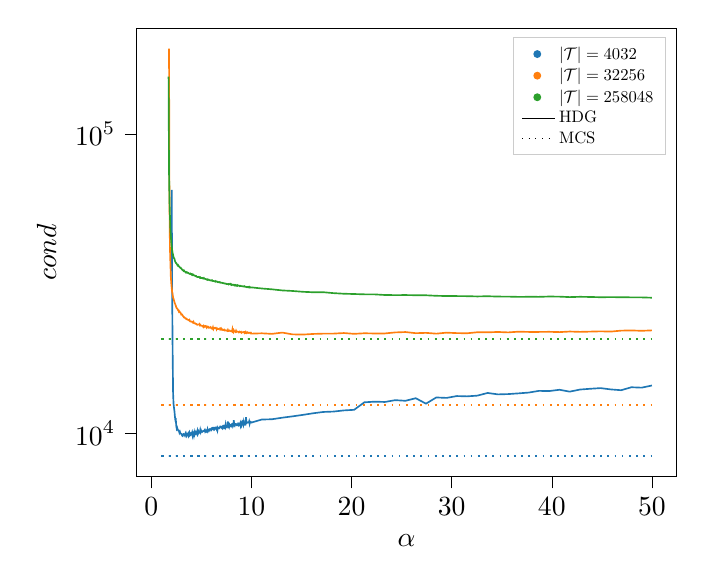
\begin{tikzpicture}

\definecolor{color0}{rgb}{0.12156862745098,0.466666666666667,0.705882352941177}
\definecolor{color1}{rgb}{1,0.498039215686275,0.0549019607843137}
\definecolor{color2}{rgb}{0.172549019607843,0.627450980392157,0.172549019607843}

\pgfplotsset{
    legend image with text/.style={
        legend image code/.code={%
            \node[anchor=center] at (0.3cm,0cm) {#1};
        }
    },
  }
  
\begin{axis}[
legend cell align={left},
legend style={fill opacity=0.8, draw opacity=1, text opacity=1, draw=white!80!black,
  nodes = {scale=.6, transform shape}},
log basis y={10},
tick align=outside,
tick pos=left,
x grid style={white!69.0196078431373!black},
xlabel={\(\displaystyle \alpha\)},
% ylabel={\(\displaystyle \kappa\)},
ylabel={\({\operatorname{cond}}\)},
xmin=-1.45, xmax=52.45,
xtick style={color=black},
y grid style={white!69.0196078431373!black},
ymin=7159.6500072001, ymax=225826.216509126,
ymode=log,
legend image post style={scale=.7},
ytick style={color=black},
ytick={100,1000,10000,100000,1000000,10000000},
yticklabels={
  \(\displaystyle {10^{2}}\),
  \(\displaystyle {10^{3}}\),
  \(\displaystyle {10^{4}}\),
  \(\displaystyle {10^{5}}\),
  \(\displaystyle {10^{6}}\),
  \(\displaystyle {10^{7}}\)
}
]

\addplot [semithick, color0, dotted, forget plot]
table {%
1 8375.73288281204
1.04522613065327 8375.73288281204
1.09045226130653 8375.73288281204
1.1356783919598 8375.73288281204
1.18090452261307 8375.73288281204
1.22613065326633 8375.73288281204
1.2713567839196 8375.73288281204
1.31658291457286 8375.73288281204
1.36180904522613 8375.73288281204
1.4070351758794 8375.73288281204
1.45226130653266 8375.73288281204
1.49748743718593 8375.73288281204
1.5427135678392 8375.73288281204
1.58793969849246 8375.73288281204
1.63316582914573 8375.73288281204
1.67839195979899 8375.73288281204
1.72361809045226 8375.73288281204
1.76884422110553 8375.73288281204
1.81407035175879 8375.73288281204
1.85929648241206 8375.73288281204
1.90452261306533 8375.73288281204
1.94974874371859 8375.73288281204
1.99497487437186 8375.73288281204
2.04020100502513 8375.73288281204
2.08542713567839 8375.73288281204
2.13065326633166 8375.73288281204
2.17587939698492 8375.73288281204
2.22110552763819 8375.73288281204
2.26633165829146 8375.73288281204
2.31155778894472 8375.73288281204
2.35678391959799 8375.73288281204
2.40201005025126 8375.73288281204
2.44723618090452 8375.73288281204
2.49246231155779 8375.73288281204
2.53768844221106 8375.73288281204
2.58291457286432 8375.73288281204
2.62814070351759 8375.73288281204
2.67336683417085 8375.73288281204
2.71859296482412 8375.73288281204
2.76381909547739 8375.73288281204
2.80904522613065 8375.73288281204
2.85427135678392 8375.73288281204
2.89949748743719 8375.73288281204
2.94472361809045 8375.73288281204
2.98994974874372 8375.73288281204
3.03517587939699 8375.73288281204
3.08040201005025 8375.73288281204
3.12562814070352 8375.73288281204
3.17085427135678 8375.73288281204
3.21608040201005 8375.73288281204
3.26130653266332 8375.73288281204
3.30653266331658 8375.73288281204
3.35175879396985 8375.73288281204
3.39698492462312 8375.73288281204
3.44221105527638 8375.73288281204
3.48743718592965 8375.73288281204
3.53266331658291 8375.73288281204
3.57788944723618 8375.73288281204
3.62311557788945 8375.73288281204
3.66834170854271 8375.73288281204
3.71356783919598 8375.73288281204
3.75879396984925 8375.73288281204
3.80402010050251 8375.73288281204
3.84924623115578 8375.73288281204
3.89447236180905 8375.73288281204
3.93969849246231 8375.73288281204
3.98492462311558 8375.73288281204
4.03015075376884 8375.73288281204
4.07537688442211 8375.73288281204
4.12060301507538 8375.73288281204
4.16582914572864 8375.73288281204
4.21105527638191 8375.73288281204
4.25628140703518 8375.73288281204
4.30150753768844 8375.73288281204
4.34673366834171 8375.73288281204
4.39195979899498 8375.73288281204
4.43718592964824 8375.73288281204
4.48241206030151 8375.73288281204
4.52763819095477 8375.73288281204
4.57286432160804 8375.73288281204
4.61809045226131 8375.73288281204
4.66331658291457 8375.73288281204
4.70854271356784 8375.73288281204
4.75376884422111 8375.73288281204
4.79899497487437 8375.73288281204
4.84422110552764 8375.73288281204
4.8894472361809 8375.73288281204
4.93467336683417 8375.73288281204
4.97989949748744 8375.73288281204
5.0251256281407 8375.73288281204
5.07035175879397 8375.73288281204
5.11557788944724 8375.73288281204
5.1608040201005 8375.73288281204
5.20603015075377 8375.73288281204
5.25125628140704 8375.73288281204
5.2964824120603 8375.73288281204
5.34170854271357 8375.73288281204
5.38693467336683 8375.73288281204
5.4321608040201 8375.73288281204
5.47738693467337 8375.73288281204
5.52261306532663 8375.73288281204
5.5678391959799 8375.73288281204
5.61306532663317 8375.73288281204
5.65829145728643 8375.73288281204
5.7035175879397 8375.73288281204
5.74874371859296 8375.73288281204
5.79396984924623 8375.73288281204
5.8391959798995 8375.73288281204
5.88442211055276 8375.73288281204
5.92964824120603 8375.73288281204
5.9748743718593 8375.73288281204
6.02010050251256 8375.73288281204
6.06532663316583 8375.73288281204
6.1105527638191 8375.73288281204
6.15577889447236 8375.73288281204
6.20100502512563 8375.73288281204
6.24623115577889 8375.73288281204
6.29145728643216 8375.73288281204
6.33668341708543 8375.73288281204
6.38190954773869 8375.73288281204
6.42713567839196 8375.73288281204
6.47236180904523 8375.73288281204
6.51758793969849 8375.73288281204
6.56281407035176 8375.73288281204
6.60804020100502 8375.73288281204
6.65326633165829 8375.73288281204
6.69849246231156 8375.73288281204
6.74371859296482 8375.73288281204
6.78894472361809 8375.73288281204
6.83417085427136 8375.73288281204
6.87939698492462 8375.73288281204
6.92462311557789 8375.73288281204
6.96984924623116 8375.73288281204
7.01507537688442 8375.73288281204
7.06030150753769 8375.73288281204
7.10552763819095 8375.73288281204
7.15075376884422 8375.73288281204
7.19597989949749 8375.73288281204
7.24120603015075 8375.73288281204
7.28643216080402 8375.73288281204
7.33165829145729 8375.73288281204
7.37688442211055 8375.73288281204
7.42211055276382 8375.73288281204
7.46733668341709 8375.73288281204
7.51256281407035 8375.73288281204
7.55778894472362 8375.73288281204
7.60301507537688 8375.73288281204
7.64824120603015 8375.73288281204
7.69346733668342 8375.73288281204
7.73869346733668 8375.73288281204
7.78391959798995 8375.73288281204
7.82914572864322 8375.73288281204
7.87437185929648 8375.73288281204
7.91959798994975 8375.73288281204
7.96482412060302 8375.73288281204
8.01005025125628 8375.73288281204
8.05527638190955 8375.73288281204
8.10050251256281 8375.73288281204
8.14572864321608 8375.73288281204
8.19095477386935 8375.73288281204
8.23618090452261 8375.73288281204
8.28140703517588 8375.73288281204
8.32663316582915 8375.73288281204
8.37185929648241 8375.73288281204
8.41708542713568 8375.73288281204
8.46231155778895 8375.73288281204
8.50753768844221 8375.73288281204
8.55276381909548 8375.73288281204
8.59798994974874 8375.73288281204
8.64321608040201 8375.73288281204
8.68844221105528 8375.73288281204
8.73366834170854 8375.73288281204
8.77889447236181 8375.73288281204
8.82412060301507 8375.73288281204
8.86934673366834 8375.73288281204
8.91457286432161 8375.73288281204
8.95979899497488 8375.73288281204
9.00502512562814 8375.73288281204
9.05025125628141 8375.73288281204
9.09547738693467 8375.73288281204
9.14070351758794 8375.73288281204
9.18592964824121 8375.73288281204
9.23115577889447 8375.73288281204
9.27638190954774 8375.73288281204
9.321608040201 8375.73288281204
9.36683417085427 8375.73288281204
9.41206030150754 8375.73288281204
9.4572864321608 8375.73288281204
9.50251256281407 8375.73288281204
9.54773869346734 8375.73288281204
9.5929648241206 8375.73288281204
9.63819095477387 8375.73288281204
9.68341708542714 8375.73288281204
9.7286432160804 8375.73288281204
9.77386934673367 8375.73288281204
9.81909547738693 8375.73288281204
9.8643216080402 8375.73288281204
9.90954773869347 8375.73288281204
9.95477386934673 8375.73288281204
10 8375.73288281204
11.025641025641 8375.73288281204
12.0512820512821 8375.73288281204
13.0769230769231 8375.73288281204
14.1025641025641 8375.73288281204
15.1282051282051 8375.73288281204
16.1538461538462 8375.73288281204
17.1794871794872 8375.73288281204
18.2051282051282 8375.73288281204
19.2307692307692 8375.73288281204
20.2564102564103 8375.73288281204
21.2820512820513 8375.73288281204
22.3076923076923 8375.73288281204
23.3333333333333 8375.73288281204
24.3589743589744 8375.73288281204
25.3846153846154 8375.73288281204
26.4102564102564 8375.73288281204
27.4358974358974 8375.73288281204
28.4615384615385 8375.73288281204
29.4871794871795 8375.73288281204
30.5128205128205 8375.73288281204
31.5384615384615 8375.73288281204
32.5641025641026 8375.73288281204
33.5897435897436 8375.73288281204
34.6153846153846 8375.73288281204
35.6410256410256 8375.73288281204
36.6666666666667 8375.73288281204
37.6923076923077 8375.73288281204
38.7179487179487 8375.73288281204
39.7435897435897 8375.73288281204
40.7692307692308 8375.73288281204
41.7948717948718 8375.73288281204
42.8205128205128 8375.73288281204
43.8461538461538 8375.73288281204
44.8717948717949 8375.73288281204
45.8974358974359 8375.73288281204
46.9230769230769 8375.73288281204
47.9487179487179 8375.73288281204
48.974358974359 8375.73288281204
50 8375.73288281204
};

\addplot [semithick, color0, forget plot]
table {%
2.04020100502513 64995.3109247881
2.08542713567839 28386.507062522
2.13065326633166 18565.8353628636
2.17587939698492 13560.1754506261
2.22110552763819 12504.4044833549
2.26633165829146 12158.0470862759
2.31155778894472 11836.4904255309
2.35678391959799 11367.9327676037
2.40201005025126 11056.9571507777
2.44723618090452 11090.0580177186
2.49246231155779 10564.4388828359
2.53768844221106 10347.7868276963
2.58291457286432 10428.3202300872
2.62814070351759 10306.4875216724
2.67336683417085 10237.1247322767
2.71859296482412 10168.0593004942
2.76381909547739 10151.2616195426
2.80904522613065 10023.9598331485
2.85427135678392 10111.2013239367
2.89949748743719 10001.715053117
2.94472361809045 9962.2382775974
2.98994974874372 9945.78011106269
3.03517587939699 9902.42790358886
3.08040201005025 9803.057752411
3.12562814070352 9778.44226785343
3.17085427135678 9892.45553760851
3.21608040201005 9926.50625185411
3.26130653266332 9901.34241107388
3.30653266331658 9877.22128262886
3.35175879396985 9812.1976693309
3.39698492462312 9963.82383065821
3.44221105527638 10030.1115018488
3.48743718592965 9913.5802966819
3.53266331658291 9797.73599889626
3.57788944723618 9891.72340712821
3.62311557788945 9911.425816093
3.66834170854271 9973.88974064123
3.71356783919598 9824.70280854481
3.75879396984925 9946.3042078155
3.80402010050251 10039.8309891772
3.84924623115578 9864.22289574785
3.89447236180905 9933.19092461315
3.93969849246231 9883.59543194856
3.98492462311558 9992.29163290331
4.03015075376884 9977.88041442986
4.07537688442211 10068.2555662905
4.12060301507538 9858.47042158672
4.16582914572864 10065.5641690743
4.21105527638191 10048.6694151063
4.25628140703518 9848.89170633102
4.30150753768844 10060.2574931169
4.34673366834171 9914.92204512277
4.39195979899498 10011.0311809388
4.43718592964824 10087.5949362549
4.48241206030151 9960.58170396963
4.52763819095477 9980.92168169179
4.57286432160804 9911.48557682457
4.61809045226131 10151.4589419612
4.66331658291457 9998.56723138012
4.70854271356784 10114.4269480456
4.75376884422111 10009.9818575834
4.79899497487437 10051.3023867965
4.84422110552764 10054.4722183285
4.8894472361809 10245.0355469214
4.93467336683417 10079.3964508179
4.97989949748744 10187.4250163129
5.0251256281407 10097.3321270022
5.07035175879397 10088.2372203341
5.11557788944724 10131.0313729636
5.1608040201005 10160.3888416901
5.20603015075377 10147.3834982469
5.25125628140704 10157.2901548865
5.2964824120603 10206.5970940997
5.34170854271357 10257.2747753697
5.38693467336683 10097.4431889909
5.4321608040201 10142.5634105409
5.47738693467337 10181.1748134874
5.52261306532663 10099.9871157671
5.5678391959799 10112.4882122826
5.61306532663317 10287.0948070408
5.65829145728643 10144.9296757144
5.7035175879397 10221.8680595438
5.74874371859296 10242.7599594029
5.79396984924623 10279.502191442
5.8391959798995 10212.8501082178
5.88442211055276 10304.0227231786
5.92964824120603 10312.6101774001
5.9748743718593 10349.2754711971
6.02010050251256 10263.424398127
6.06532663316583 10319.6096666913
6.1105527638191 10379.6403120715
6.15577889447236 10338.9580574659
6.20100502512563 10430.3124105339
6.24623115577889 10425.9159007821
6.29145728643216 10273.3428928822
6.33668341708543 10312.473514559
6.38190954773869 10397.9757110239
6.42713567839196 10443.803739757
6.47236180904523 10433.7967861043
6.51758793969849 10320.7161381307
6.56281407035176 10411.7607478029
6.60804020100502 10239.6473033615
6.65326633165829 10438.1406661024
6.69849246231156 10410.2332784666
6.74371859296482 10396.4167968051
6.78894472361809 10381.7457933028
6.83417085427136 10434.3040548549
6.87939698492462 10524.7007905941
6.92462311557789 10525.3563233212
6.96984924623116 10453.6984271746
7.01507537688442 10422.2940125203
7.06030150753769 10472.748867809
7.10552763819095 10374.279314188
7.15075376884422 10433.4041842383
7.19597989949749 10590.2316642898
7.24120603015075 10596.1287839732
7.28643216080402 10444.3004187979
7.33165829145729 10512.0920365954
7.37688442211055 10438.8348250351
7.42211055276382 10668.7537877192
7.46733668341709 10444.48482035
7.51256281407035 10465.4167095907
7.55778894472362 10494.1271258646
7.60301507537688 10501.9005302545
7.64824120603015 10929.9410535097
7.69346733668342 10567.195367909
7.73869346733668 10642.7958496861
7.78391959798995 10507.5879833436
7.82914572864322 10641.040903984
7.87437185929648 10546.5481223144
7.91959798994975 10539.2773017771
7.96482412060302 10520.8521894178
8.01005025125628 10685.6924469893
8.05527638190955 10716.0241952576
8.10050251256281 10665.8835050612
8.14572864321608 10535.0679239667
8.19095477386935 10617.4053286478
8.23618090452261 11047.2765318694
8.28140703517588 10641.5123691675
8.32663316582915 10585.4952735562
8.37185929648241 10723.3588171325
8.41708542713568 10727.7043034574
8.46231155778895 10676.4270666514
8.50753768844221 10641.1617188363
8.55276381909548 10690.082543124
8.59798994974874 10655.1518565503
8.64321608040201 10724.8505147315
8.68844221105528 10640.2172321855
8.73366834170854 10712.0979657296
8.77889447236181 10644.233251759
8.82412060301507 10689.3361423238
8.86934673366834 10779.7131937145
8.91457286432161 10604.3603666175
8.95979899497488 10795.8380816801
9.00502512562814 10648.6665508092
9.05025125628141 10818.0624171491
9.09547738693467 10898.677046474
9.14070351758794 10775.844378673
9.18592964824121 10654.9133521522
9.23115577889447 10901.2085797941
9.27638190954774 10703.438969996
9.321608040201 10663.4516253932
9.36683417085427 10655.091390973
9.41206030150754 10671.4727256198
9.4572864321608 11311.1003235788
9.50251256281407 10822.0512260764
9.54773869346734 10867.8785681719
9.5929648241206 10839.8268319985
9.63819095477387 10862.320800602
9.68341708542714 10843.1625790415
9.7286432160804 10835.9414554502
9.77386934673367 10955.2560542399
9.81909547738693 10754.2085434045
9.8643216080402 10916.4955973723
9.90954773869347 10874.563054831
9.95477386934673 10889.6370385233
10 10846.1989383146
11.025641025641 11100.6087568416
12.0512820512821 11126.2184158795
13.0769230769231 11260.2130198873
14.1025641025641 11377.4344391991
15.1282051282051 11505.7422710624
16.1538461538462 11647.9035022509
17.1794871794872 11768.1242012887
18.2051282051282 11803.9196783649
19.2307692307692 11907.4309370254
20.2564102564103 11964.4943392015
21.2820512820513 12677.2082796565
22.3076923076923 12738.5247830179
23.3333333333333 12709.7707617151
24.3589743589744 12888.2351753807
25.3846153846154 12823.977575353
26.4102564102564 13080.250058728
27.4358974358974 12544.6388757996
28.4615384615385 13158.5953653624
29.4871794871795 13112.5171937582
30.5128205128205 13301.186378816
31.5384615384615 13270.7009307508
32.5641025641026 13344.1592720746
33.5897435897436 13623.0405911834
34.6153846153846 13473.7188143915
35.6410256410256 13504.9382364367
36.6666666666667 13577.8839731013
37.6923076923077 13662.4167533384
38.7179487179487 13842.5481955731
39.7435897435897 13822.1137832145
40.7692307692308 13961.2752038645
41.7948717948718 13759.10847736
42.8205128205128 13986.2143562314
43.8461538461538 14068.1906507642
44.8717948717949 14140.7739911501
45.8974358974359 13998.0804106193
46.9230769230769 13912.8009789987
47.9487179487179 14233.875349339
48.974358974359 14189.8102385292
50 14427.8322215117
};

\addplot [semithick, color1, dotted, forget plot]
table {%
1 12403.9475730826
1.04522613065327 12403.9475730826
1.09045226130653 12403.9475730826
1.1356783919598 12403.9475730826
1.18090452261307 12403.9475730826
1.22613065326633 12403.9475730826
1.2713567839196 12403.9475730826
1.31658291457286 12403.9475730826
1.36180904522613 12403.9475730826
1.4070351758794 12403.9475730826
1.45226130653266 12403.9475730826
1.49748743718593 12403.9475730826
1.5427135678392 12403.9475730826
1.58793969849246 12403.9475730826
1.63316582914573 12403.9475730826
1.67839195979899 12403.9475730826
1.72361809045226 12403.9475730826
1.76884422110553 12403.9475730826
1.81407035175879 12403.9475730826
1.85929648241206 12403.9475730826
1.90452261306533 12403.9475730826
1.94974874371859 12403.9475730826
1.99497487437186 12403.9475730826
2.04020100502513 12403.9475730826
2.08542713567839 12403.9475730826
2.13065326633166 12403.9475730826
2.17587939698492 12403.9475730826
2.22110552763819 12403.9475730826
2.26633165829146 12403.9475730826
2.31155778894472 12403.9475730826
2.35678391959799 12403.9475730826
2.40201005025126 12403.9475730826
2.44723618090452 12403.9475730826
2.49246231155779 12403.9475730826
2.53768844221106 12403.9475730826
2.58291457286432 12403.9475730826
2.62814070351759 12403.9475730826
2.67336683417085 12403.9475730826
2.71859296482412 12403.9475730826
2.76381909547739 12403.9475730826
2.80904522613065 12403.9475730826
2.85427135678392 12403.9475730826
2.89949748743719 12403.9475730826
2.94472361809045 12403.9475730826
2.98994974874372 12403.9475730826
3.03517587939699 12403.9475730826
3.08040201005025 12403.9475730826
3.12562814070352 12403.9475730826
3.17085427135678 12403.9475730826
3.21608040201005 12403.9475730826
3.26130653266332 12403.9475730826
3.30653266331658 12403.9475730826
3.35175879396985 12403.9475730826
3.39698492462312 12403.9475730826
3.44221105527638 12403.9475730826
3.48743718592965 12403.9475730826
3.53266331658291 12403.9475730826
3.57788944723618 12403.9475730826
3.62311557788945 12403.9475730826
3.66834170854271 12403.9475730826
3.71356783919598 12403.9475730826
3.75879396984925 12403.9475730826
3.80402010050251 12403.9475730826
3.84924623115578 12403.9475730826
3.89447236180905 12403.9475730826
3.93969849246231 12403.9475730826
3.98492462311558 12403.9475730826
4.03015075376884 12403.9475730826
4.07537688442211 12403.9475730826
4.12060301507538 12403.9475730826
4.16582914572864 12403.9475730826
4.21105527638191 12403.9475730826
4.25628140703518 12403.9475730826
4.30150753768844 12403.9475730826
4.34673366834171 12403.9475730826
4.39195979899498 12403.9475730826
4.43718592964824 12403.9475730826
4.48241206030151 12403.9475730826
4.52763819095477 12403.9475730826
4.57286432160804 12403.9475730826
4.61809045226131 12403.9475730826
4.66331658291457 12403.9475730826
4.70854271356784 12403.9475730826
4.75376884422111 12403.9475730826
4.79899497487437 12403.9475730826
4.84422110552764 12403.9475730826
4.8894472361809 12403.9475730826
4.93467336683417 12403.9475730826
4.97989949748744 12403.9475730826
5.0251256281407 12403.9475730826
5.07035175879397 12403.9475730826
5.11557788944724 12403.9475730826
5.1608040201005 12403.9475730826
5.20603015075377 12403.9475730826
5.25125628140704 12403.9475730826
5.2964824120603 12403.9475730826
5.34170854271357 12403.9475730826
5.38693467336683 12403.9475730826
5.4321608040201 12403.9475730826
5.47738693467337 12403.9475730826
5.52261306532663 12403.9475730826
5.5678391959799 12403.9475730826
5.61306532663317 12403.9475730826
5.65829145728643 12403.9475730826
5.7035175879397 12403.9475730826
5.74874371859296 12403.9475730826
5.79396984924623 12403.9475730826
5.8391959798995 12403.9475730826
5.88442211055276 12403.9475730826
5.92964824120603 12403.9475730826
5.9748743718593 12403.9475730826
6.02010050251256 12403.9475730826
6.06532663316583 12403.9475730826
6.1105527638191 12403.9475730826
6.15577889447236 12403.9475730826
6.20100502512563 12403.9475730826
6.24623115577889 12403.9475730826
6.29145728643216 12403.9475730826
6.33668341708543 12403.9475730826
6.38190954773869 12403.9475730826
6.42713567839196 12403.9475730826
6.47236180904523 12403.9475730826
6.51758793969849 12403.9475730826
6.56281407035176 12403.9475730826
6.60804020100502 12403.9475730826
6.65326633165829 12403.9475730826
6.69849246231156 12403.9475730826
6.74371859296482 12403.9475730826
6.78894472361809 12403.9475730826
6.83417085427136 12403.9475730826
6.87939698492462 12403.9475730826
6.92462311557789 12403.9475730826
6.96984924623116 12403.9475730826
7.01507537688442 12403.9475730826
7.06030150753769 12403.9475730826
7.10552763819095 12403.9475730826
7.15075376884422 12403.9475730826
7.19597989949749 12403.9475730826
7.24120603015075 12403.9475730826
7.28643216080402 12403.9475730826
7.33165829145729 12403.9475730826
7.37688442211055 12403.9475730826
7.42211055276382 12403.9475730826
7.46733668341709 12403.9475730826
7.51256281407035 12403.9475730826
7.55778894472362 12403.9475730826
7.60301507537688 12403.9475730826
7.64824120603015 12403.9475730826
7.69346733668342 12403.9475730826
7.73869346733668 12403.9475730826
7.78391959798995 12403.9475730826
7.82914572864322 12403.9475730826
7.87437185929648 12403.9475730826
7.91959798994975 12403.9475730826
7.96482412060302 12403.9475730826
8.01005025125628 12403.9475730826
8.05527638190955 12403.9475730826
8.10050251256281 12403.9475730826
8.14572864321608 12403.9475730826
8.19095477386935 12403.9475730826
8.23618090452261 12403.9475730826
8.28140703517588 12403.9475730826
8.32663316582915 12403.9475730826
8.37185929648241 12403.9475730826
8.41708542713568 12403.9475730826
8.46231155778895 12403.9475730826
8.50753768844221 12403.9475730826
8.55276381909548 12403.9475730826
8.59798994974874 12403.9475730826
8.64321608040201 12403.9475730826
8.68844221105528 12403.9475730826
8.73366834170854 12403.9475730826
8.77889447236181 12403.9475730826
8.82412060301507 12403.9475730826
8.86934673366834 12403.9475730826
8.91457286432161 12403.9475730826
8.95979899497488 12403.9475730826
9.00502512562814 12403.9475730826
9.05025125628141 12403.9475730826
9.09547738693467 12403.9475730826
9.14070351758794 12403.9475730826
9.18592964824121 12403.9475730826
9.23115577889447 12403.9475730826
9.27638190954774 12403.9475730826
9.321608040201 12403.9475730826
9.36683417085427 12403.9475730826
9.41206030150754 12403.9475730826
9.4572864321608 12403.9475730826
9.50251256281407 12403.9475730826
9.54773869346734 12403.9475730826
9.5929648241206 12403.9475730826
9.63819095477387 12403.9475730826
9.68341708542714 12403.9475730826
9.7286432160804 12403.9475730826
9.77386934673367 12403.9475730826
9.81909547738693 12403.9475730826
9.8643216080402 12403.9475730826
9.90954773869347 12403.9475730826
9.95477386934673 12403.9475730826
10 12403.9475730826
11.025641025641 12403.9475730826
12.0512820512821 12403.9475730826
13.0769230769231 12403.9475730826
14.1025641025641 12403.9475730826
15.1282051282051 12403.9475730826
16.1538461538462 12403.9475730826
17.1794871794872 12403.9475730826
18.2051282051282 12403.9475730826
19.2307692307692 12403.9475730826
20.2564102564103 12403.9475730826
21.2820512820513 12403.9475730826
22.3076923076923 12403.9475730826
23.3333333333333 12403.9475730826
24.3589743589744 12403.9475730826
25.3846153846154 12403.9475730826
26.4102564102564 12403.9475730826
27.4358974358974 12403.9475730826
28.4615384615385 12403.9475730826
29.4871794871795 12403.9475730826
30.5128205128205 12403.9475730826
31.5384615384615 12403.9475730826
32.5641025641026 12403.9475730826
33.5897435897436 12403.9475730826
34.6153846153846 12403.9475730826
35.6410256410256 12403.9475730826
36.6666666666667 12403.9475730826
37.6923076923077 12403.9475730826
38.7179487179487 12403.9475730826
39.7435897435897 12403.9475730826
40.7692307692308 12403.9475730826
41.7948717948718 12403.9475730826
42.8205128205128 12403.9475730826
43.8461538461538 12403.9475730826
44.8717948717949 12403.9475730826
45.8974358974359 12403.9475730826
46.9230769230769 12403.9475730826
47.9487179487179 12403.9475730826
48.974358974359 12403.9475730826
50 12403.9475730826
};

\addplot [semithick, color1, forget plot]
table {%
1.76884422110553 193038.232627197
1.81407035175879 58094.742976004
1.85929648241206 41648.2279944724
1.90452261306533 37217.8554314865
1.94974874371859 33332.3672719412
1.99497487437186 31674.6164573244
2.04020100502513 30523.955934079
2.08542713567839 29588.3677226043
2.13065326633166 29034.5716510825
2.17587939698492 28380.4611553167
2.22110552763819 28162.5093403657
2.26633165829146 27763.2305733698
2.31155778894472 27427.033894789
2.35678391959799 27149.8692414193
2.40201005025126 26903.9704165024
2.44723618090452 26667.7499994352
2.49246231155779 26332.3764035487
2.53768844221106 26151.7464731995
2.58291457286432 26099.8055273246
2.62814070351759 25983.059036337
2.67336683417085 25748.4893500037
2.71859296482412 25757.2095258967
2.76381909547739 25424.6833244342
2.80904522613065 25485.0796431111
2.85427135678392 25330.7736581318
2.89949748743719 25333.527075314
2.94472361809045 25156.4268911203
2.98994974874372 24906.1089858686
3.03517587939699 24931.5730990678
3.08040201005025 24917.2868021359
3.12562814070352 24731.0974534678
3.17085427135678 24611.1613625392
3.21608040201005 24504.2631051798
3.26130653266332 24367.8148342936
3.30653266331658 24391.2222035591
3.35175879396985 24276.6805782404
3.39698492462312 24219.8076536208
3.44221105527638 24109.8825693419
3.48743718592965 24133.2298455004
3.53266331658291 24033.3858869486
3.57788944723618 24019.7421934211
3.62311557788945 23946.6721827819
3.66834170854271 23911.4521319514
3.71356783919598 23889.3495930571
3.75879396984925 23831.3645097462
3.80402010050251 23913.3781770149
3.84924623115578 23698.71880746
3.89447236180905 23611.1726395981
3.93969849246231 23616.1366657228
3.98492462311558 23608.547083236
4.03015075376884 23594.9653925398
4.07537688442211 23543.7785016967
4.12060301507538 23427.7131580126
4.16582914572864 23469.14907294
4.21105527638191 23579.5847671197
4.25628140703518 23328.7210176824
4.30150753768844 23285.7593488096
4.34673366834171 23258.5185156511
4.39195979899498 23274.2463235564
4.43718592964824 23179.1010125943
4.48241206030151 23174.2040292979
4.52763819095477 23149.026775198
4.57286432160804 23031.559164013
4.61809045226131 23042.7130421007
4.66331658291457 23044.8863754241
4.70854271356784 23055.6211809815
4.75376884422111 23060.2160358463
4.79899497487437 23153.3349067981
4.84422110552764 22948.6099249963
4.8894472361809 23023.2920487293
4.93467336683417 22918.5410265314
4.97989949748744 22843.5333763837
5.0251256281407 22834.4418734331
5.07035175879397 22830.010090049
5.11557788944724 22811.9951003817
5.1608040201005 22705.6723644296
5.20603015075377 22828.4204680729
5.25125628140704 22652.7574824459
5.2964824120603 22787.1790175314
5.34170854271357 22721.6623709098
5.38693467336683 22789.8889334925
5.4321608040201 22821.0786349665
5.47738693467337 22654.4476070142
5.52261306532663 22525.1823874637
5.5678391959799 22673.2393194003
5.61306532663317 22611.6498260566
5.65829145728643 22700.3487366121
5.7035175879397 22633.6627866955
5.74874371859296 22508.400947533
5.79396984924623 22547.9826333858
5.8391959798995 22516.3907512712
5.88442211055276 22502.1803540373
5.92964824120603 22597.0967061845
5.9748743718593 22477.6156160701
6.02010050251256 22414.0984569666
6.06532663316583 22333.7015997208
6.1105527638191 22345.5447506563
6.15577889447236 22579.8748000275
6.20100502512563 22278.9791886015
6.24623115577889 22444.1317193448
6.29145728643216 22435.6888949673
6.33668341708543 22493.6395721785
6.38190954773869 22514.8766021117
6.42713567839196 22447.3597162152
6.47236180904523 22435.1362400225
6.51758793969849 22226.0447673217
6.56281407035176 22395.6304276235
6.60804020100502 22287.6272681569
6.65326633165829 22268.3154922134
6.69849246231156 22293.1762550007
6.74371859296482 22303.5824471784
6.78894472361809 22336.5462486314
6.83417085427136 22387.5450210215
6.87939698492462 22194.8150782803
6.92462311557789 22271.0446919424
6.96984924623116 22376.9844718866
7.01507537688442 22183.5523693303
7.06030150753769 22143.5377094202
7.10552763819095 22224.6841579469
7.15075376884422 22187.0162258161
7.19597989949749 22111.400758953
7.24120603015075 22092.5494878419
7.28643216080402 22166.7789393164
7.33165829145729 22046.57416991
7.37688442211055 22086.9770179231
7.42211055276382 22044.7238422657
7.46733668341709 22056.6865565616
7.51256281407035 22000.7599849726
7.55778894472362 21973.5798097823
7.60301507537688 21944.7998719436
7.64824120603015 22132.9037622364
7.69346733668342 21957.8011495213
7.73869346733668 21956.1104617091
7.78391959798995 21996.8787473201
7.82914572864322 22039.1992475973
7.87437185929648 21959.3437360585
7.91959798994975 21932.9870676836
7.96482412060302 21916.7490514817
8.01005025125628 21954.3115521337
8.05527638190955 21879.2391303517
8.10050251256281 22238.884321211
8.14572864321608 21795.7150201803
8.19095477386935 21716.9424291131
8.23618090452261 22059.0935735787
8.28140703517588 21922.8917900771
8.32663316582915 21927.632168133
8.37185929648241 21865.8400584669
8.41708542713568 21792.080802658
8.46231155778895 21996.6657504686
8.50753768844221 21810.6973581339
8.55276381909548 21854.2984831333
8.59798994974874 21861.0394839594
8.64321608040201 21830.1506138633
8.68844221105528 21765.5907155681
8.73366834170854 21706.8405520838
8.77889447236181 21732.5408063068
8.82412060301507 21825.5015425811
8.86934673366834 21751.0672048567
8.91457286432161 21757.851991157
8.95979899497488 21803.8786553719
9.00502512562814 21658.813380556
9.05025125628141 21720.3522266514
9.09547738693467 21746.472439381
9.14070351758794 21716.7511279105
9.18592964824121 21720.5228310904
9.23115577889447 21784.6171938708
9.27638190954774 21793.7818832885
9.321608040201 21623.318581461
9.36683417085427 21714.0450768741
9.41206030150754 21796.8468561976
9.4572864321608 21590.7452009389
9.50251256281407 21573.2335405227
9.54773869346734 21609.304273793
9.5929648241206 21731.6117770672
9.63819095477387 21671.7880900111
9.68341708542714 21647.6144051076
9.7286432160804 21608.4237066722
9.77386934673367 21660.9894375296
9.81909547738693 21670.1333298848
9.8643216080402 21668.9013200898
9.90954773869347 21579.6146631437
9.95477386934673 21642.9112106855
10 21506.755629305
11.025641025641 21563.2623139906
12.0512820512821 21469.7061615056
13.0769230769231 21681.1289614775
14.1025641025641 21386.0475192342
15.1282051282051 21351.1944720687
16.1538461538462 21456.1633629973
17.1794871794872 21506.0594554969
18.2051282051282 21512.5918568869
19.2307692307692 21606.4746671397
20.2564102564103 21473.4745567127
21.2820512820513 21569.3882529578
22.3076923076923 21533.5787602312
23.3333333333333 21540.8283779765
24.3589743589744 21709.5155735543
25.3846153846154 21772.8195110099
26.4102564102564 21583.1996202037
27.4358974358974 21636.2027623082
28.4615384615385 21503.0071680326
29.4871794871795 21669.351288983
30.5128205128205 21593.9718358806
31.5384615384615 21570.1774957925
32.5641025641026 21739.6517308262
33.5897435897436 21724.8832004788
34.6153846153846 21785.2037475788
35.6410256410256 21713.9650282511
36.6666666666667 21831.0146045775
37.6923076923077 21792.2733374503
38.7179487179487 21793.6152445698
39.7435897435897 21810.9407965831
40.7692307692308 21763.1507479621
41.7948717948718 21857.6132198938
42.8205128205128 21802.6816761484
43.8461538461538 21846.3798383651
44.8717948717949 21890.6779957494
45.8974358974359 21850.3333302589
46.9230769230769 22009.9165239694
47.9487179487179 22042.9635432588
48.974358974359 21980.9223241076
50 22052.1286323671
};

\addplot [semithick, color2, dotted, forget plot]
table {%
1 20626.8403867383
1.04522613065327 20626.8403867383
1.09045226130653 20626.8403867383
1.1356783919598 20626.8403867383
1.18090452261307 20626.8403867383
1.22613065326633 20626.8403867383
1.2713567839196 20626.8403867383
1.31658291457286 20626.8403867383
1.36180904522613 20626.8403867383
1.4070351758794 20626.8403867383
1.45226130653266 20626.8403867383
1.49748743718593 20626.8403867383
1.5427135678392 20626.8403867383
1.58793969849246 20626.8403867383
1.63316582914573 20626.8403867383
1.67839195979899 20626.8403867383
1.72361809045226 20626.8403867383
1.76884422110553 20626.8403867383
1.81407035175879 20626.8403867383
1.85929648241206 20626.8403867383
1.90452261306533 20626.8403867383
1.94974874371859 20626.8403867383
1.99497487437186 20626.8403867383
2.04020100502513 20626.8403867383
2.08542713567839 20626.8403867383
2.13065326633166 20626.8403867383
2.17587939698492 20626.8403867383
2.22110552763819 20626.8403867383
2.26633165829146 20626.8403867383
2.31155778894472 20626.8403867383
2.35678391959799 20626.8403867383
2.40201005025126 20626.8403867383
2.44723618090452 20626.8403867383
2.49246231155779 20626.8403867383
2.53768844221106 20626.8403867383
2.58291457286432 20626.8403867383
2.62814070351759 20626.8403867383
2.67336683417085 20626.8403867383
2.71859296482412 20626.8403867383
2.76381909547739 20626.8403867383
2.80904522613065 20626.8403867383
2.85427135678392 20626.8403867383
2.89949748743719 20626.8403867383
2.94472361809045 20626.8403867383
2.98994974874372 20626.8403867383
3.03517587939699 20626.8403867383
3.08040201005025 20626.8403867383
3.12562814070352 20626.8403867383
3.17085427135678 20626.8403867383
3.21608040201005 20626.8403867383
3.26130653266332 20626.8403867383
3.30653266331658 20626.8403867383
3.35175879396985 20626.8403867383
3.39698492462312 20626.8403867383
3.44221105527638 20626.8403867383
3.48743718592965 20626.8403867383
3.53266331658291 20626.8403867383
3.57788944723618 20626.8403867383
3.62311557788945 20626.8403867383
3.66834170854271 20626.8403867383
3.71356783919598 20626.8403867383
3.75879396984925 20626.8403867383
3.80402010050251 20626.8403867383
3.84924623115578 20626.8403867383
3.89447236180905 20626.8403867383
3.93969849246231 20626.8403867383
3.98492462311558 20626.8403867383
4.03015075376884 20626.8403867383
4.07537688442211 20626.8403867383
4.12060301507538 20626.8403867383
4.16582914572864 20626.8403867383
4.21105527638191 20626.8403867383
4.25628140703518 20626.8403867383
4.30150753768844 20626.8403867383
4.34673366834171 20626.8403867383
4.39195979899498 20626.8403867383
4.43718592964824 20626.8403867383
4.48241206030151 20626.8403867383
4.52763819095477 20626.8403867383
4.57286432160804 20626.8403867383
4.61809045226131 20626.8403867383
4.66331658291457 20626.8403867383
4.70854271356784 20626.8403867383
4.75376884422111 20626.8403867383
4.79899497487437 20626.8403867383
4.84422110552764 20626.8403867383
4.8894472361809 20626.8403867383
4.93467336683417 20626.8403867383
4.97989949748744 20626.8403867383
5.0251256281407 20626.8403867383
5.07035175879397 20626.8403867383
5.11557788944724 20626.8403867383
5.1608040201005 20626.8403867383
5.20603015075377 20626.8403867383
5.25125628140704 20626.8403867383
5.2964824120603 20626.8403867383
5.34170854271357 20626.8403867383
5.38693467336683 20626.8403867383
5.4321608040201 20626.8403867383
5.47738693467337 20626.8403867383
5.52261306532663 20626.8403867383
5.5678391959799 20626.8403867383
5.61306532663317 20626.8403867383
5.65829145728643 20626.8403867383
5.7035175879397 20626.8403867383
5.74874371859296 20626.8403867383
5.79396984924623 20626.8403867383
5.8391959798995 20626.8403867383
5.88442211055276 20626.8403867383
5.92964824120603 20626.8403867383
5.9748743718593 20626.8403867383
6.02010050251256 20626.8403867383
6.06532663316583 20626.8403867383
6.1105527638191 20626.8403867383
6.15577889447236 20626.8403867383
6.20100502512563 20626.8403867383
6.24623115577889 20626.8403867383
6.29145728643216 20626.8403867383
6.33668341708543 20626.8403867383
6.38190954773869 20626.8403867383
6.42713567839196 20626.8403867383
6.47236180904523 20626.8403867383
6.51758793969849 20626.8403867383
6.56281407035176 20626.8403867383
6.60804020100502 20626.8403867383
6.65326633165829 20626.8403867383
6.69849246231156 20626.8403867383
6.74371859296482 20626.8403867383
6.78894472361809 20626.8403867383
6.83417085427136 20626.8403867383
6.87939698492462 20626.8403867383
6.92462311557789 20626.8403867383
6.96984924623116 20626.8403867383
7.01507537688442 20626.8403867383
7.06030150753769 20626.8403867383
7.10552763819095 20626.8403867383
7.15075376884422 20626.8403867383
7.19597989949749 20626.8403867383
7.24120603015075 20626.8403867383
7.28643216080402 20626.8403867383
7.33165829145729 20626.8403867383
7.37688442211055 20626.8403867383
7.42211055276382 20626.8403867383
7.46733668341709 20626.8403867383
7.51256281407035 20626.8403867383
7.55778894472362 20626.8403867383
7.60301507537688 20626.8403867383
7.64824120603015 20626.8403867383
7.69346733668342 20626.8403867383
7.73869346733668 20626.8403867383
7.78391959798995 20626.8403867383
7.82914572864322 20626.8403867383
7.87437185929648 20626.8403867383
7.91959798994975 20626.8403867383
7.96482412060302 20626.8403867383
8.01005025125628 20626.8403867383
8.05527638190955 20626.8403867383
8.10050251256281 20626.8403867383
8.14572864321608 20626.8403867383
8.19095477386935 20626.8403867383
8.23618090452261 20626.8403867383
8.28140703517588 20626.8403867383
8.32663316582915 20626.8403867383
8.37185929648241 20626.8403867383
8.41708542713568 20626.8403867383
8.46231155778895 20626.8403867383
8.50753768844221 20626.8403867383
8.55276381909548 20626.8403867383
8.59798994974874 20626.8403867383
8.64321608040201 20626.8403867383
8.68844221105528 20626.8403867383
8.73366834170854 20626.8403867383
8.77889447236181 20626.8403867383
8.82412060301507 20626.8403867383
8.86934673366834 20626.8403867383
8.91457286432161 20626.8403867383
8.95979899497488 20626.8403867383
9.00502512562814 20626.8403867383
9.05025125628141 20626.8403867383
9.09547738693467 20626.8403867383
9.14070351758794 20626.8403867383
9.18592964824121 20626.8403867383
9.23115577889447 20626.8403867383
9.27638190954774 20626.8403867383
9.321608040201 20626.8403867383
9.36683417085427 20626.8403867383
9.41206030150754 20626.8403867383
9.4572864321608 20626.8403867383
9.50251256281407 20626.8403867383
9.54773869346734 20626.8403867383
9.5929648241206 20626.8403867383
9.63819095477387 20626.8403867383
9.68341708542714 20626.8403867383
9.7286432160804 20626.8403867383
9.77386934673367 20626.8403867383
9.81909547738693 20626.8403867383
9.8643216080402 20626.8403867383
9.90954773869347 20626.8403867383
9.95477386934673 20626.8403867383
10 20626.8403867383
11.025641025641 20626.8403867383
12.0512820512821 20626.8403867383
13.0769230769231 20626.8403867383
14.1025641025641 20626.8403867383
15.1282051282051 20626.8403867383
16.1538461538462 20626.8403867383
17.1794871794872 20626.8403867383
18.2051282051282 20626.8403867383
19.2307692307692 20626.8403867383
20.2564102564103 20626.8403867383
21.2820512820513 20626.8403867383
22.3076923076923 20626.8403867383
23.3333333333333 20626.8403867383
24.3589743589744 20626.8403867383
25.3846153846154 20626.8403867383
26.4102564102564 20626.8403867383
27.4358974358974 20626.8403867383
28.4615384615385 20626.8403867383
29.4871794871795 20626.8403867383
30.5128205128205 20626.8403867383
31.5384615384615 20626.8403867383
32.5641025641026 20626.8403867383
33.5897435897436 20626.8403867383
34.6153846153846 20626.8403867383
35.6410256410256 20626.8403867383
36.6666666666667 20626.8403867383
37.6923076923077 20626.8403867383
38.7179487179487 20626.8403867383
39.7435897435897 20626.8403867383
40.7692307692308 20626.8403867383
41.7948717948718 20626.8403867383
42.8205128205128 20626.8403867383
43.8461538461538 20626.8403867383
44.8717948717949 20626.8403867383
45.8974358974359 20626.8403867383
46.9230769230769 20626.8403867383
47.9487179487179 20626.8403867383
48.974358974359 20626.8403867383
50 20626.8403867383
};

\addplot [semithick, color2, forget plot]
table {%
1.72361809045226 155667.689678908
1.76884422110553 74965.8421249181
1.81407035175879 59988.7545349186
1.85929648241206 53461.3007373607
1.90452261306533 47839.8234142235
1.94974874371859 45490.0249037382
1.99497487437186 43421.9778653281
2.04020100502513 41841.9534944475
2.08542713567839 40877.0588082292
2.13065326633166 40006.3684960895
2.17587939698492 39361.6973315437
2.22110552763819 38795.2752263606
2.26633165829146 38453.9585900928
2.31155778894472 38252.2613814192
2.35678391959799 37698.2341907201
2.40201005025126 37361.5323514043
2.44723618090452 37098.8041005031
2.49246231155779 37060.3304559038
2.53768844221106 36809.446815081
2.58291457286432 36603.6510295627
2.62814070351759 36359.7436025565
2.67336683417085 36452.8061615938
2.71859296482412 36149.8121524993
2.76381909547739 36117.2610448805
2.80904522613065 35932.2076389551
2.85427135678392 35845.3440924435
2.89949748743719 35685.4376733375
2.94472361809045 35716.0402072871
2.98994974874372 35485.0657022236
3.03517587939699 35373.5411960847
3.08040201005025 35216.915860346
3.12562814070352 35039.9944713357
3.17085427135678 35079.3014431458
3.21608040201005 34905.8556890025
3.26130653266332 34971.0537189605
3.30653266331658 34677.1713868922
3.35175879396985 34682.8262700286
3.39698492462312 34660.8178209141
3.44221105527638 34476.9226104928
3.48743718592965 34585.8206615593
3.53266331658291 34537.3431675811
3.57788944723618 34375.0094859576
3.62311557788945 34429.1248326876
3.66834170854271 34289.6938258095
3.71356783919598 34297.2736021602
3.75879396984925 34185.2837956223
3.80402010050251 34073.4511325174
3.84924623115578 34108.7514034206
3.89447236180905 34162.0979448321
3.93969849246231 34005.9172715305
3.98492462311558 33958.5700015064
4.03015075376884 34024.5321343474
4.07537688442211 33752.1397541709
4.12060301507538 33722.6159724115
4.16582914572864 33886.98546174
4.21105527638191 33736.1879960918
4.25628140703518 33704.2622537728
4.30150753768844 33689.8073894992
4.34673366834171 33566.8632933885
4.39195979899498 33565.7113231713
4.43718592964824 33485.7674236442
4.48241206030151 33507.7870115767
4.52763819095477 33334.1479733911
4.57286432160804 33296.741310925
4.61809045226131 33262.9483144502
4.66331658291457 33247.703814233
4.70854271356784 33263.5301489182
4.75376884422111 33311.622645859
4.79899497487437 33256.2356177981
4.84422110552764 33092.3495167834
4.8894472361809 33182.6316203379
4.93467336683417 32988.9505457408
4.97989949748744 33009.4746276568
5.0251256281407 33045.9583559606
5.07035175879397 33029.6019157139
5.11557788944724 33000.8662831616
5.1608040201005 32866.991358874
5.20603015075377 32845.7824097021
5.25125628140704 32993.4966201789
5.2964824120603 32793.664010434
5.34170854271357 32806.8767512337
5.38693467336683 32781.4171676581
5.4321608040201 32712.1452904485
5.47738693467337 32709.5673046226
5.52261306532663 32703.6640395906
5.5678391959799 32566.6251794657
5.61306532663317 32648.003926611
5.65829145728643 32535.2815116131
5.7035175879397 32609.4951883459
5.74874371859296 32570.6907770599
5.79396984924623 32503.8534542232
5.8391959798995 32448.7346249966
5.88442211055276 32427.1791846295
5.92964824120603 32380.3967328155
5.9748743718593 32431.6524042024
6.02010050251256 32364.6679365799
6.06532663316583 32437.8971546936
6.1105527638191 32289.9837210985
6.15577889447236 32227.8552733859
6.20100502512563 32249.1918028049
6.24623115577889 32253.4111887675
6.29145728643216 32213.7477609941
6.33668341708543 32157.5663918569
6.38190954773869 32105.789695694
6.42713567839196 32228.709199096
6.47236180904523 32094.0756115419
6.51758793969849 32141.7813500525
6.56281407035176 32130.9391951521
6.60804020100502 32008.2843657823
6.65326633165829 31950.0252298875
6.69849246231156 31998.2257283137
6.74371859296482 31954.7982617949
6.78894472361809 31982.7842054598
6.83417085427136 31901.3090548686
6.87939698492462 31948.8121110596
6.92462311557789 31838.197834688
6.96984924623116 31838.2822473629
7.01507537688442 31799.9018458322
7.06030150753769 31813.5225236377
7.10552763819095 31757.3732900765
7.15075376884422 31764.874667319
7.19597989949749 31682.6794803139
7.24120603015075 31693.2291605912
7.28643216080402 31684.3784851803
7.33165829145729 31615.3489423561
7.37688442211055 31646.1365832678
7.42211055276382 31583.2683908442
7.46733668341709 31596.1805772379
7.51256281407035 31500.6363452701
7.55778894472362 31479.2718736962
7.60301507537688 31478.8272011551
7.64824120603015 31523.2176215269
7.69346733668342 31506.6942285436
7.73869346733668 31409.5012056206
7.78391959798995 31535.3734820546
7.82914572864322 31476.3819723282
7.87437185929648 31476.414375076
7.91959798994975 31551.6726512571
7.96482412060302 31337.7538996708
8.01005025125628 31419.3845802961
8.05527638190955 31272.1009301165
8.10050251256281 31330.6906377259
8.14572864321608 31353.7064686297
8.19095477386935 31348.6124229403
8.23618090452261 31287.601119578
8.28140703517588 31184.5211273488
8.32663316582915 31270.3900019233
8.37185929648241 31160.1030433403
8.41708542713568 31277.9660109469
8.46231155778895 31182.6910242519
8.50753768844221 31212.5737102471
8.55276381909548 31092.1568617362
8.59798994974874 31220.8099180127
8.64321608040201 31098.9449109138
8.68844221105528 31165.150032544
8.73366834170854 31124.7564105175
8.77889447236181 31097.9372813309
8.82412060301507 31009.8972412973
8.86934673366834 31094.7195074364
8.91457286432161 31014.5653499004
8.95979899497488 31041.7322885346
9.00502512562814 30998.3736299304
9.05025125628141 30987.9904598267
9.09547738693467 31006.4170176653
9.14070351758794 30944.2077550288
9.18592964824121 30902.2625936034
9.23115577889447 30937.2623138365
9.27638190954774 31019.3166720533
9.321608040201 30933.3584965909
9.36683417085427 30820.503530122
9.41206030150754 30868.0015634711
9.4572864321608 30844.1313251486
9.50251256281407 30824.4828754665
9.54773869346734 30752.3404301797
9.5929648241206 30806.5704328264
9.63819095477387 30760.9934498824
9.68341708542714 30808.1545102253
9.7286432160804 30718.1893575356
9.77386934673367 30838.3615349704
9.81909547738693 30692.1831973617
9.8643216080402 30754.1845744205
9.90954773869347 30687.5627518624
9.95477386934673 30698.2892629265
10 30705.3250576646
11.025641025641 30449.1986322469
12.0512820512821 30251.1885432839
13.0769230769231 29993.9741947915
14.1025641025641 29871.5862979155
15.1282051282051 29682.367369099
16.1538461538462 29577.9859891585
17.1794871794872 29582.6363449988
18.2051282051282 29376.985757398
19.2307692307692 29240.8831123768
20.2564102564103 29176.9052231413
21.2820512820513 29106.4442900686
22.3076923076923 29094.9383355792
23.3333333333333 28960.2220551178
24.3589743589744 28930.5051997072
25.3846153846154 28946.3226834516
26.4102564102564 28908.5859585105
27.4358974358974 28895.3369059365
28.4615384615385 28782.1739459447
29.4871794871795 28728.6420685371
30.5128205128205 28719.1529845667
31.5384615384615 28695.2918879034
32.5641025641026 28639.1599832123
33.5897435897436 28684.4508872866
34.6153846153846 28610.4784710812
35.6410256410256 28599.3698660222
36.6666666666667 28542.9530631448
37.6923076923077 28558.617873629
38.7179487179487 28552.0724232749
39.7435897435897 28622.0294426834
40.7692307692308 28593.5777599385
41.7948717948718 28491.8390551469
42.8205128205128 28559.5059719814
43.8461538461538 28522.9117063944
44.8717948717949 28462.190719027
45.8974358974359 28491.4527128956
46.9230769230769 28461.3267290533
47.9487179487179 28438.4270945259
48.974358974359 28427.9469758048
50 28358.0962030684
};

\addlegendimage{legend image code/.code={%
            \node[shape=circle, fill, color=color0, opacity=1] at (0.2cm,0cm) {};
          }};
\addlegendentry{$|\mathcal{T}|=4032$}
\addlegendimage{legend image code/.code={%
            \node[shape=circle, fill, color=color1, opacity=1] at (0.2cm,0cm) {};
          }};
\addlegendentry{$|\mathcal{T}|=32256$}
\addlegendimage{legend image code/.code={%
            \node[shape=circle, fill, color=color2, opacity=1] at (0.2cm,0cm) {};
          }};
\addlegendentry{$|\mathcal{T}|=258048$}

\addlegendimage{no markers, black}
\addlegendentry{HDG}
\addlegendimage{no markers, dotted, black}
\addlegendentry{MCS}
% \addlegendimage{legend image code/.code={%
            % \node[shape=circle, scale=.8, color=black, opacity=1] at (0.1cm,0cm) {};
          % }};


\end{axis}

\end{tikzpicture}

    }
  \caption{Approximate condition numbers of the corresponding $A$
    blocks of the HDG (solid lines) and the MCS (dotted lines in the
    same color) method on different meshes. Different values of
    $\alpha$ on the x axis and approximate condition number ($\operatorname{cond}$) on the y axis. }
  \label{fig::kappas}
\end{figure}


%%% Local Variables:
%%% mode: latex
%%% TeX-master: arxiv
%%% End:
